\section{Efficiency}
\label{sec:RKst_efficiency}

The efficiency for each of the decay channels is calculated according to the formula
%
$$\varepsilon^{tot} = \varepsilon^{\rm geom} \cdot \varepsilon^{\rm reco|geom} \cdot \varepsilon^{\rm PID|reco} \cdot \varepsilon^{\rm trig|PID} \cdot \varepsilon^{\rm MVA|trig}\cdot \varepsilon^{\rm BCM|MVA},$$
%
where the first term is the efficiency to have final state particles in the LHCb detector 
acceptance; the second term ($\varepsilon^{\rm reco|geom}$) carries information about the reconstruction and pre-selection efficiency;
%(we keep these together given that boundaries between them are completely artificial).
the third ($\varepsilon^{\rm PID|reco}$) corresponds to the efficiency of the PID requirements;
the fourth ($\varepsilon^{\rm trig|PID}$) handles the trigger efficiency for those events which are selected by the pre-selection 
process; and, finally, the latter two terms deal with the efficiency of the neural network classifier and the BCM requirement.
Geometric, reconstruction, trigger, MVA and BCM efficiencies are evaluated using simulated data samples with the trigger efficiency
for $\Bz\to\Kstarz\jpsi$ being cross-checked using the data-driven TISTOS method as described in Sec.~\ref{sec:Lb_trigger_eff}.
The PID efficiency is calculated with a data-driven method as described in Sec.~\ref{sec:RKst_pid_eff}.

%All absolute efficiencies for the muon and electron rare channels are separately listed in Tab.~\ref{tab:RKst_AbsEff}
%for the central and high \qsq intervals and 
Absolute efficiencies for the muon and electron normalisation channels are reported in Tab.~\ref{tab:AbsEff_jpsi}
and relative efficiencies between the rare and resonant channels, 
$\varepsilon^{\ell\ell}/\varepsilon^{\jpsi(\ell\ell)}$, are listed in Tab.~\ref{tab:RKst_RelEff};
these are the efficiencies which are used in the fit.

%
%($\varepsilon(\Bz\to\Kstar ee)/\varepsilon(\Bz\to\Kstar(\jpsi\to ee))$)/($\varepsilon(\Bz\to\Kstar \mumu)/\varepsilon(\Bz\to\Kstar(\jpsi\to \mumu))$).
%Systematic uncertainties for relative efficiencies take into account that some effects are correlated between two decays.
%In table \ref{tab:AbsEffs} are reported absolute efficiencies
%for the electron and muon channels in the \qsq bin $1 < q^2 < 6$ \gevgevcccc.
%
%
%Finally, Tab.~\ref{tab:double_rel_eff} reports double-ratios of the efficiencies
%for the $ee$ and $\mu\mu$ channels, $[\varepsilon(ee)/\varepsilon(\jpsi (ee))] / [\varepsilon(\mu\mu)/\varepsilon(\jpsi(\mu\mu))]$.
%
%In particular the latter table contains the total double-relative
%efficiency, $\varepsilon_tot^{drel} = \pm $, which is used for the final result extraction.

\begin{table}[h!]
\centering
\caption{Absolute efficiencies for the resonant $\mu\mu$ and $ee$ channels. 
For the latter, the efficiency is shown for each of the three L0 categories considered.}
\renewcommand\arraystretch{1.25}
\begin{tabular}{c|c|c|c|c}
\multirow{2}{*}{\boldmath{$\varepsilon$}} 	&  \boldmath{$\mu\mu$} 	& \multicolumn {3}{c}{\boldmath{$ee$}} \\ \cline{2-5}
	  & &  L0E 	& L0H 	& L0I \\ \hline
$\varepsilon^{\rm geom}$  & $ 0.1598  \pm  0.0005 $ & \multicolumn{3}{c}{$ 0.1589  \pm  0.0005 $} \\
$\varepsilon^{\rm reco|geom}$  & $ 0.0947  \pm  0.0001 $ & \multicolumn{3}{c}{$ 0.0603  \pm  0.0001 $} \\
$\varepsilon^{\rm PID|reco}$  & $ 0.8148  \pm  0.0000 $ & \multicolumn{3}{c}{$ 0.8222  \pm  0.0000 $} \\
\hline
$\varepsilon^{\rm trig|PID}$  & $ 0.7511  \pm  0.0005 $ & $ 0.1939  \pm  0.0005 $ & $ 0.0163  \pm  0.0002 $ & $ 0.0707  \pm  0.0003 $ \\
$\varepsilon^{\rm MVA|trig}$   & $ 0.8944  \pm  0.0004 $ & $ 0.8597  \pm  0.0007 $ & $ 0.8983  \pm  0.0006 $ & $ 0.8276  \pm  0.0017 $ \\
\hline
$\varepsilon^{\rm Total}$   & $ 0.0083  \pm  0.0000 $ & $ 0.0013  \pm  0.0000 $ & $ 0.0001  \pm  0.0000 $ & $ 0.0005  \pm  0.0000 $ \\
\end{tabular}
\label{tab:AbsEff_jpsi}
\end{table}

%\begin{landscape}

\begin{table}
\centering
\caption{Relative efficiencies, $\varepsilon^{\rm rel} = \varepsilon^{\ell\ell} / \varepsilon^{\jpsi(\ell\ell)}$,
for the $\mu\mu$ and $ee$ channels in the low-, central- and high-\qsq intervals.}
\renewcommand\arraystretch{1.25}
\begin{tabular}{c|c|c|c|c}
\multirow{2}{*}{\textbf{\boldmath{$\varepsilon$}}}
 & \boldmath{$\mu\mu$} & \multicolumn {3}{c}{\boldmath{$ee$}} \\ \cline{2-5}
 & & L0E & L0H & L0I \\

\hline
\multicolumn{5}{c}{\textbf{low-}{\boldmath\qsq}} \\ \hline
$\varepsilon^{\rm geom}$  & $ 1.0200 \pm 0.0091$ & \multicolumn{3}{c}{$ 1.0429 \pm 0.0084$}  \\
$\varepsilon^{\rm reco|geom}$  & $ 0.1309 \pm 0.0010$ & \multicolumn{3}{c}{$ 0.1961 \pm 0.0007$}  \\
$\varepsilon^{\rm PID|reco}$  & $ 0.9861 \pm 0.0003$ & \multicolumn{3}{c}{$ 0.9718 \pm 0.0001$}  \\
\hline
$\varepsilon^{\rm trig|PID}$  & $ 0.8103 \pm 0.0048 $ & $ 0.6478 \pm 0.0058 $ & $ 2.5556 \pm 0.0455 $ & $ 1.2748 \pm 0.0139 $  \\ 
$\varepsilon^{\rm MVA|trig}$  & $ 0.9528 \pm 0.0024 $ & $ 0.9568 \pm 0.0014 $ & $ 0.9570 \pm 0.0013 $ & $ 0.9463 \pm 0.0030 $ \\
$\varepsilon^{\rm BCM|MVA}$  & -- & $ 0.9394 \pm 0.0014 $ & $ 0.9492 \pm 0.0013 $ & $ 0.9590 \pm 0.0023 $ \\
\hline
$\varepsilon^{tot}$  & $ 0.7810 \pm 0.0168 $ & $ 0.5809 \pm 0.0097 $ & $ 2.2685 \pm 0.0514 $ & $ 1.1073 \pm 0.0200 $ \\  

\hline
\multicolumn{5}{c}{\textbf{central-}{\boldmath\qsq}} \\ \hline
 $\varepsilon^{\rm geom}$  & $ 1.0200 \pm 0.0091$ & \multicolumn{3}{c}{$ 1.0429 \pm 0.0084$}  \\
$\varepsilon^{\rm reco|geom}$  & $ 0.1891 \pm 0.0012$ & \multicolumn{3}{c}{$ 0.1580 \pm 0.0006$}  \\
$\varepsilon^{\rm PID|reco}$  & $ 0.9784 \pm 0.0002$ & \multicolumn{3}{c}{$ 0.9672 \pm 0.0001$}  \\
\hline
$\varepsilon^{\rm trig|PID}$  & $ 0.8925 \pm 0.0038 $ & $ 0.7909 \pm 0.0069 $ & $ 2.1344 \pm 0.0439 $ & $ 1.1208 \pm 0.0141 $  \\ 
$\varepsilon^{\rm MVA|trig}$  & $ 0.9068 \pm 0.0024 $ & $ 0.8397 \pm 0.0024 $ & $ 0.8512 \pm 0.0022 $ & $ 0.7946 \pm 0.0054 $ \\
$\varepsilon^{\rm BCM|MVA}$  & -- & $ 0.8960 \pm 0.0020 $ & $ 0.8978 \pm 0.0020 $ & $ 0.9283 \pm 0.0037 $ \\
\hline
$\varepsilon^{tot}$  & $ 0.7171 \pm 0.0124 $ & $ 0.8145 \pm 0.0157 $ & $ 2.2235 \pm 0.0595 $ & $ 1.0542 \pm 0.0236 $ \\  

\hline
\multicolumn{5}{c}{\textbf{high-}{\boldmath\qsq}} \\ \hline
$\varepsilon^{\rm geom}$  & $ 1.0200 \pm 0.0091$ & \multicolumn{3}{c}{$ 1.0429 \pm 0.0084$}  \\
$\varepsilon^{\rm reco|geom}$  & $ 0.1172 \pm 0.0009$ & \multicolumn{3}{c}{$ 0.0530 \pm 0.0003$}  \\
$\varepsilon^{\rm PID|reco}$  & $ 1.0286 \pm 0.0001$ & \multicolumn{3}{c}{$ 1.0113 \pm 0.0002$}  \\
\hline
$\varepsilon^{\rm trig|PID}$  & $ 1.1122 \pm 0.0038 $ & $ 1.5639 \pm 0.0148 $ & -- & $ 0.8090 \pm 0.0195 $  \\ 
$\varepsilon^{\rm MVA|trig}$  & $ 0.8986 \pm 0.0027 $ & $ 0.8228 \pm 0.0036 $ & -- & $ 0.7201 \pm 0.0115 $ \\
\hline
$\varepsilon^{tot}$  & $ 0.7843 \pm 0.0155 $ & $ 0.6063 \pm 0.0131 $ & -- & $ 0.2745 \pm 0.0095 $ \\  
\end{tabular}
\label{tab:RKst_RelEff}
\end{table}


%\begin{table}
%\centering
%\caption{Relative efficiencies, $\varepsilon^{rel} = \varepsilon^{\ell\ell} / \varepsilon^{\jpsi}$,
%for the $ee$ and $\mu\mu$ channels in the central and high \qsq intervals.}
%\begin{tabular}{|c|c|c|c|c|c|c|}
%\hline \multirow{3}{*}{$\varepsilon$}  			&  \multicolumn{4}{c|}{1--6~\gevgevcccc}  				& \multicolumn {2}{c|}{15--20~\gevgevcccc}  \\ \cline{2-7}
% 				&	  $\mu\mu$  				& \multicolumn {3}{c|}{$ee$} 			&  $\mu\mu$  				& \multicolumn {1}{c|}{$ee$} \\ \cline{2-7}
%				&   &  L0E 	& L0H 	& L0I    &  	& L0E 	\\ \hline
%Geom  & $ 1.0200 \pm 0.0091$ & \multicolumn{3}{c|}{$ 1.0429 \pm 0.0084$} & $ 1.0200 \pm 0.0091$ & \multicolumn{1}{c|}{$ 1.0429 \pm 0.0084$} \\
%Reco  & $ 0.1873 \pm 0.0011$ & \multicolumn{3}{c|}{$ 0.1743 \pm 0.0006$} & $ 0.1159 \pm 0.0009$ & \multicolumn{1}{c|}{$ 0.0513 \pm 0.0003$} \\
%PID  & $ 0.9602 \pm 0.0002$ & \multicolumn{3}{c|}{$ 0.9425 \pm 0.0001$} & $ 1.0334 \pm 0.0001$ & \multicolumn{1}{c|}{$ 1.0021 \pm 0.0001$} \\
%\hline
%Trig  & $ 0.8947 \pm 0.0039 $ & $ 0.7893 \pm 0.0065 $ & $ 2.2005 \pm 0.0438 $ & $ 1.1247 \pm 0.0138 $ & $ 1.1115 \pm 0.0039 $ & $ 1.5740 \pm 0.0148 $ \\ 
%MVA  & $ 1.0143 \pm 0.0025 $ & $ 0.9841 \pm 0.0025 $ & $ 0.9495 \pm 0.0023 $ & $ 0.9838 \pm 0.0060 $ & $ 0.9223 \pm 0.0036 $ & $ 0.9812 \pm 0.0039 $ \\  
%\hline
%Tot  & $ 0.7773 \pm 0.0108 $ & $ 0.8912 \pm 0.0131 $ & $ 2.3973 \pm 0.0558 $ & $ 1.2694 \pm 0.0230 $ & $ 0.8070 \pm 0.0126 $ & $ 0.6925 \pm 0.0118 $ \\  
%\hline
%\end{tabular}\label{tab:RKst_releff}
%\end{table}

%\end{landscape}

%\begin{table}[h!]
%\centering
%\caption{Double ratios of efficiencies 
%$(\varepsilon^{ee} / \varepsilon^{\jpsi\to ee}) / (\varepsilon^{\mumu} / \varepsilon^{\jpsi\to\mumu})$
%in the central and high \qsq intervals.}
%\begin{tabular}{|c|c|c|c|c|}
%\hline
%\multirow{2}{*}{$\varepsilon$}  &  \multicolumn{3}{c|}{ 1--6~\gevgevcccc} &  \multicolumn{1}{c|}{ 15--20~\gevgevcccc } \\
%\cline{2-5} &   L0E 	& L0H 	& L0I &  L0E 	\\ \hline
%$q^2$  & \multicolumn{3}{c|}{$ 0.697 \pm 0.007 $} &  \multicolumn{1}{c|}{$ 0.770 \pm 0.010 $} \\
%Geom  & \multicolumn{3}{c|}{$ 1.022 \pm 0.012 $} &  \multicolumn{1}{c|}{$ 1.022 \pm 0.012 $} \\
%Reco  & \multicolumn{3}{c|}{$ 0.931 \pm 0.006 $} &  \multicolumn{1}{c|}{$ 0.443 \pm 0.443 $} \\
%PID  & \multicolumn{3}{c|}{$ 0.982 \pm 0.000 $} &  \multicolumn{1}{c|}{$ 0.970 \pm 0.000 $} \\
%\hline
%Trig  & $ 0.882 \pm 0.008 $ & $ 2.459 \pm 0.050 $ & $ 1.257 \pm 0.016 $ & $ 1.416 \pm 0.014 $  \\ 
%MVA  & $ 0.970 \pm 0.003 $ & $ 0.936 \pm 0.003 $ & $ 0.970 \pm 0.006 $ & $ 1.064 \pm 0.006 $  \\  
%\hline
%Tot  & $ 1.146 \pm 0.023 $ & $ 3.084 \pm 0.084 $ & $ 1.633 \pm 0.037 $ & $ 0.858 \pm 0.020 $  \\  
%\hline
%\end{tabular}
%\label{tab:double_rel_eff}
%\end{table}


\subsection{Geometric efficiency}


In order to save CPU time and disk space, simulated samples only contain decays that have
 final daughters inside the LHCb detector acceptance, which can therefore be reconstructed. 
This requires the momenta of all final state particles to be within 10 and 400 mrad 
of the beam line direction. The efficiency of this requirement is obtained using a separate
generator level simulated sample.

\subsection{Reconstruction efficiency and bin migration}
\label{sec:reco_binmig}

The reconstruction efficiency is defined as the efficiency to reconstruct
each decay channel given that its daughters are inside the geometrical acceptance
of the detector. This includes both the probability that the final particles generate
observable signatures and the efficiency of all the pre-selection requirements described
in Sec.~\ref{sec:RKst_selection}, including those intended to remove peaking backgrounds. 
%This efficiency is evaluated on simulated events
%to which the full list of weights described in Sec.~\ref{sec:RKst_weights} is applied.
The efficiency of the PID requirements are treated separately because of known deficiencies in the description 
of data by the simulation, while there are reliable data-driven methods which can be used to 
extract it (see Sec.~\ref{sec:RKst_pid_eff}).

\subsubsection{Bin migration}

Candidates produced in a given \qsq interval may be reconstructed in a different one;
this is referred to as ``bin migration'' and can be due to two different effects.
The first effect is due to the finite detector resolution that can cause candidates close to the edges
of the considered intervals to fall on the wrong side of the edge. This effect is only important
in the case where the true distributions are not flat in \qsq, as this would cause the amount of bin migration 
in the two directions to differ. The second possible source of bin migration is a systematic effect due
 to the presence of bremsstrahlung photons that cannot be recovered.
It is particularly important to take into account the bin migration for the electron channels 
because more photons are radiated from the final state and the mass resolution is worse.
Figure~\ref{fig:ee_bin_mig} shows the response matrix for simulated $\decay{\Bz}{\Kstarz\ee}$ events,
which represents the correlation between reconstructed and generated \qsq values. In the ideal case of
perfect resolution this plot would be a diagonal line and, in the case where no bias is present,
its slope would be 1. Table~\ref{tab:bin_mig} lists the net amounts of bin migration, $M_{net}$, 
in the considered \qsq intervals defined as:
%
\begin{equation}
M_{net} = N(\text{in} \to \text{in}) + N(\text{out} \to \text{in}) - N(\text{in} \to \text{out}) ,
\end{equation}
%
\noindent
where $N(\text{in} \to \text{in})$ is the number of candidates that are generated and
reconstructed inside the considered interval, $N(\text{out} \to \text{in})$ the number of 
candidates that are generated outside the interval but reconstructed inside and
$N(\text{in} \to \text{out})$ the number of candidates generated inside that fall outside.
The reconstruction efficiency is calculated comparing generated and reconstructed samples
and therefore already includes bin migration effects. Nevertheless, it is useful to single
out this component to better assess the corresponding systematic uncertainty.
%
\begin{figure}[h!]
\centering
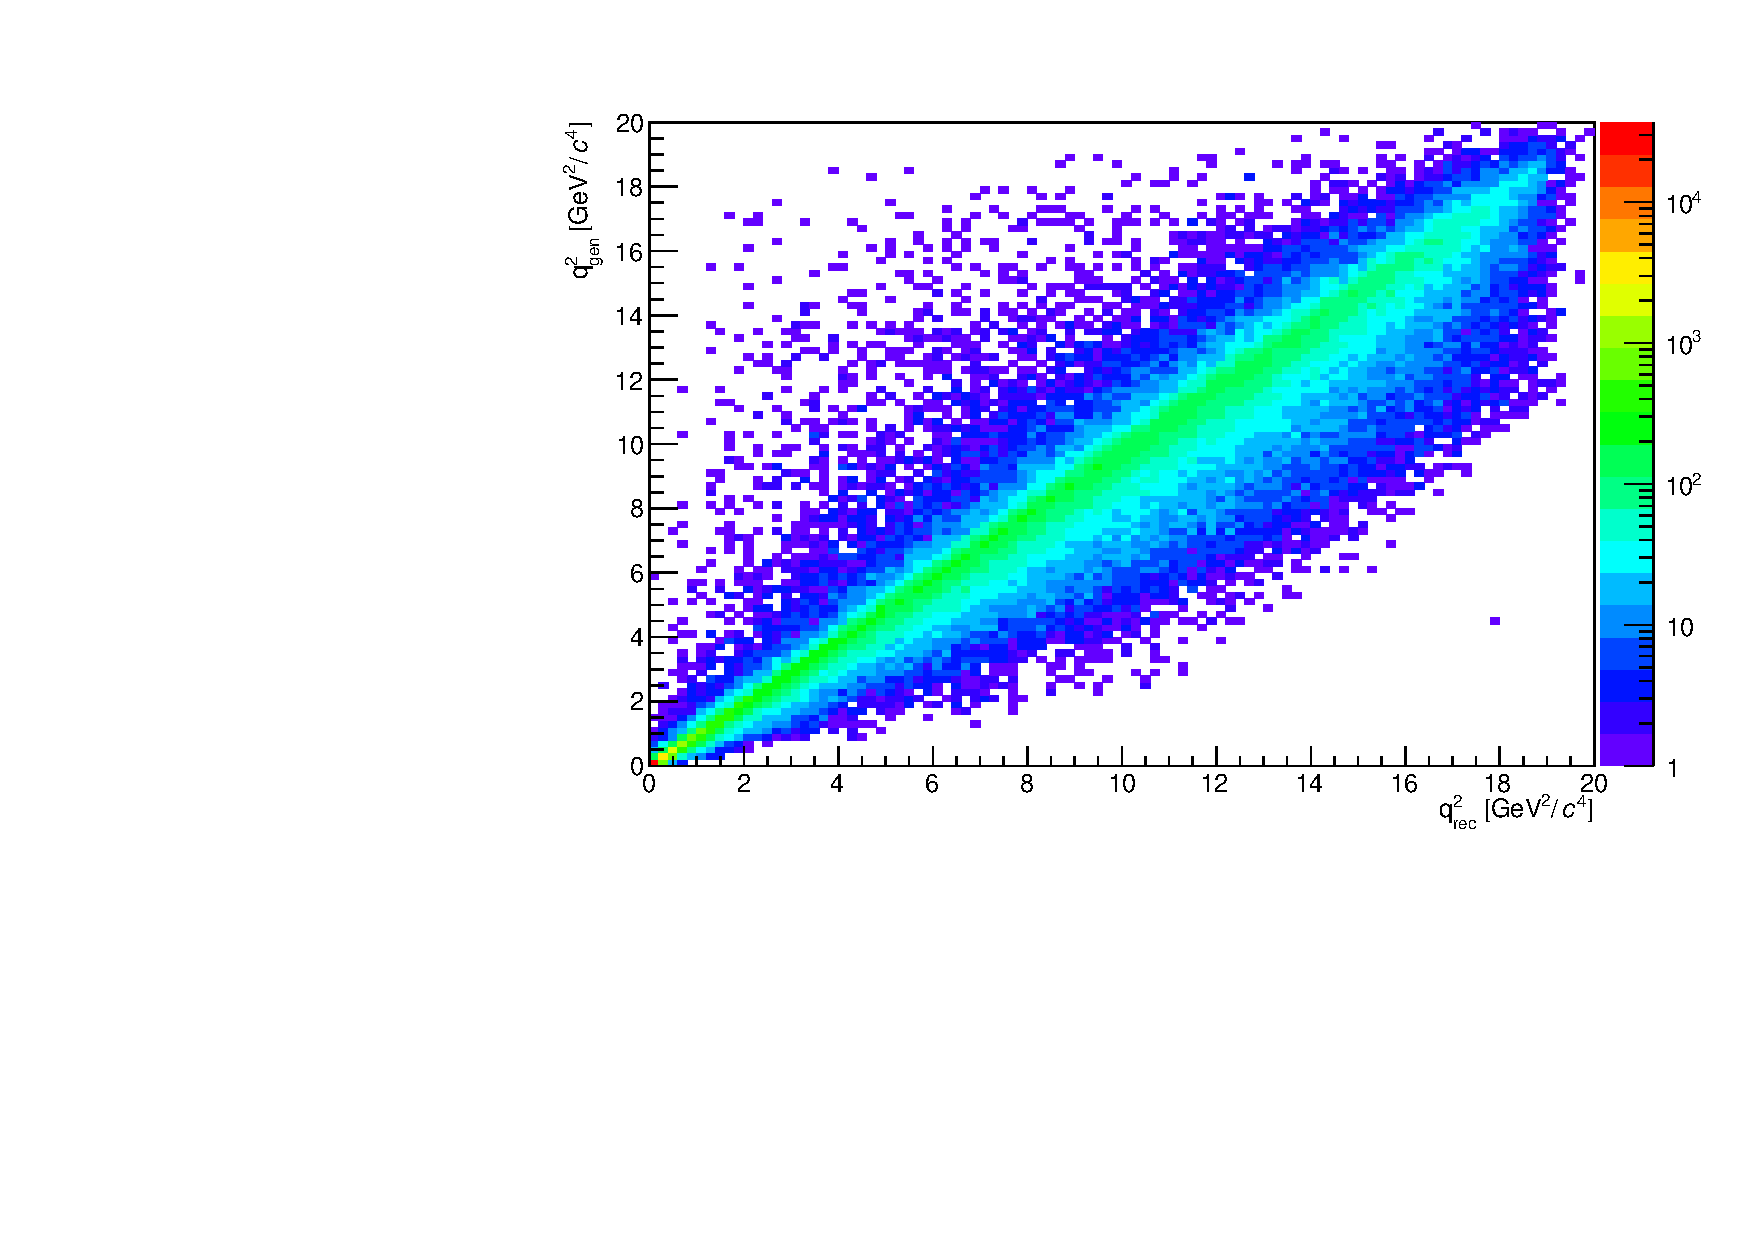
\includegraphics[width=0.85\textwidth]{RKst/figs/bin_mig.pdf}
\caption{Generated versus reconstructed \qsq for simulated $\decay{\Bz}{\Kstar\ee}$ events.}
\label{fig:ee_bin_mig}
\end{figure}
%
\begin{table}[bh]
\centering
\caption{Net bin migration amounts ($M_{net}$) in the considered \qsq intervals.
Positive values indicate ``net in", negative values ``net out".}
\begin{tabular}{$c|^c|^c|^c|^c}
\rowstyle{\bfseries}
 Sample 		& \boldmath{low-\qsq} 		& \boldmath{central-\qsq}		& \boldmath{\jpsi}   & \boldmath{high-\qsq} \\ \hline
$\mu\mu$ 	& $ 0.0002 \pm 0.0001 $ & $ -0.0021 \pm 0.0003 $ & $ 0.0032 \pm 0.0004 $ & $ -0.0012 \pm 0.0000 $ \\
$ee$ 		& $ 0.0268 \pm 0.0005 $ & $ 0.0663 \pm 0.0009 $ & $ -0.4277 \pm 0.0048 $ & $ -0.0445 \pm 0.0003 $ \\
 \end{tabular}
 \label{tab:bin_mig}
\end{table}


\subsection{PID efficiency}
\label{sec:RKst_pid_eff}

The simulation does not reliably describe particle ID variables
and therefore a data-driven method is used to obtain this efficiency component.
This is done using the \verb!PIDCalib! package described in Sec.~\ref{sec:PID_calib}.
Furthermore, the same method is used to weight the simulation in order to calculate the MVA and trigger efficiencies.
The \verb!PIDCalib! package allows the phase-space to be divided into intervals of quantities relevant for the determination 
of the PID efficiency and obtain a data-driven efficiency for each interval. For this analysis the phase-space
is divided into approximately equally populated bins of momentum and pseudorapidity of the particle under study.
Figure~\ref{fig:pid_perf_hist} shows performance tables for pions, kaons, muons and electrons.
After the efficiency tables are obtained for each particle, the total efficiency
is calculated for each candidate as the product of the four final particles efficiencies.
$\varepsilon = \varepsilon_K\cdot\varepsilon_\pi\cdot\varepsilon_{\ell_1}\cdot\varepsilon_{\ell_2}$.
Finally, as the decay channel under study generally has different kinematic distributions than the calibration sample,
the total efficiency is found by averaging over simulated events, namely
%
\begin{equation}
\varepsilon^{\rm PID} = \frac{1}{N} \sum_i^N \varepsilon_K(p_K^i,\eta_K^i) \cdot \varepsilon_\pi(p_\pi^i,\eta_\pi^i) \cdot \varepsilon_\ell(p_{\ell_1}^i,\eta_{\ell_1}^i) \cdot \varepsilon_K(p_{\ell_2}^i,\eta_{\ell_2}^i).
\end{equation}
%
\begin{figure}[h!]
\centering
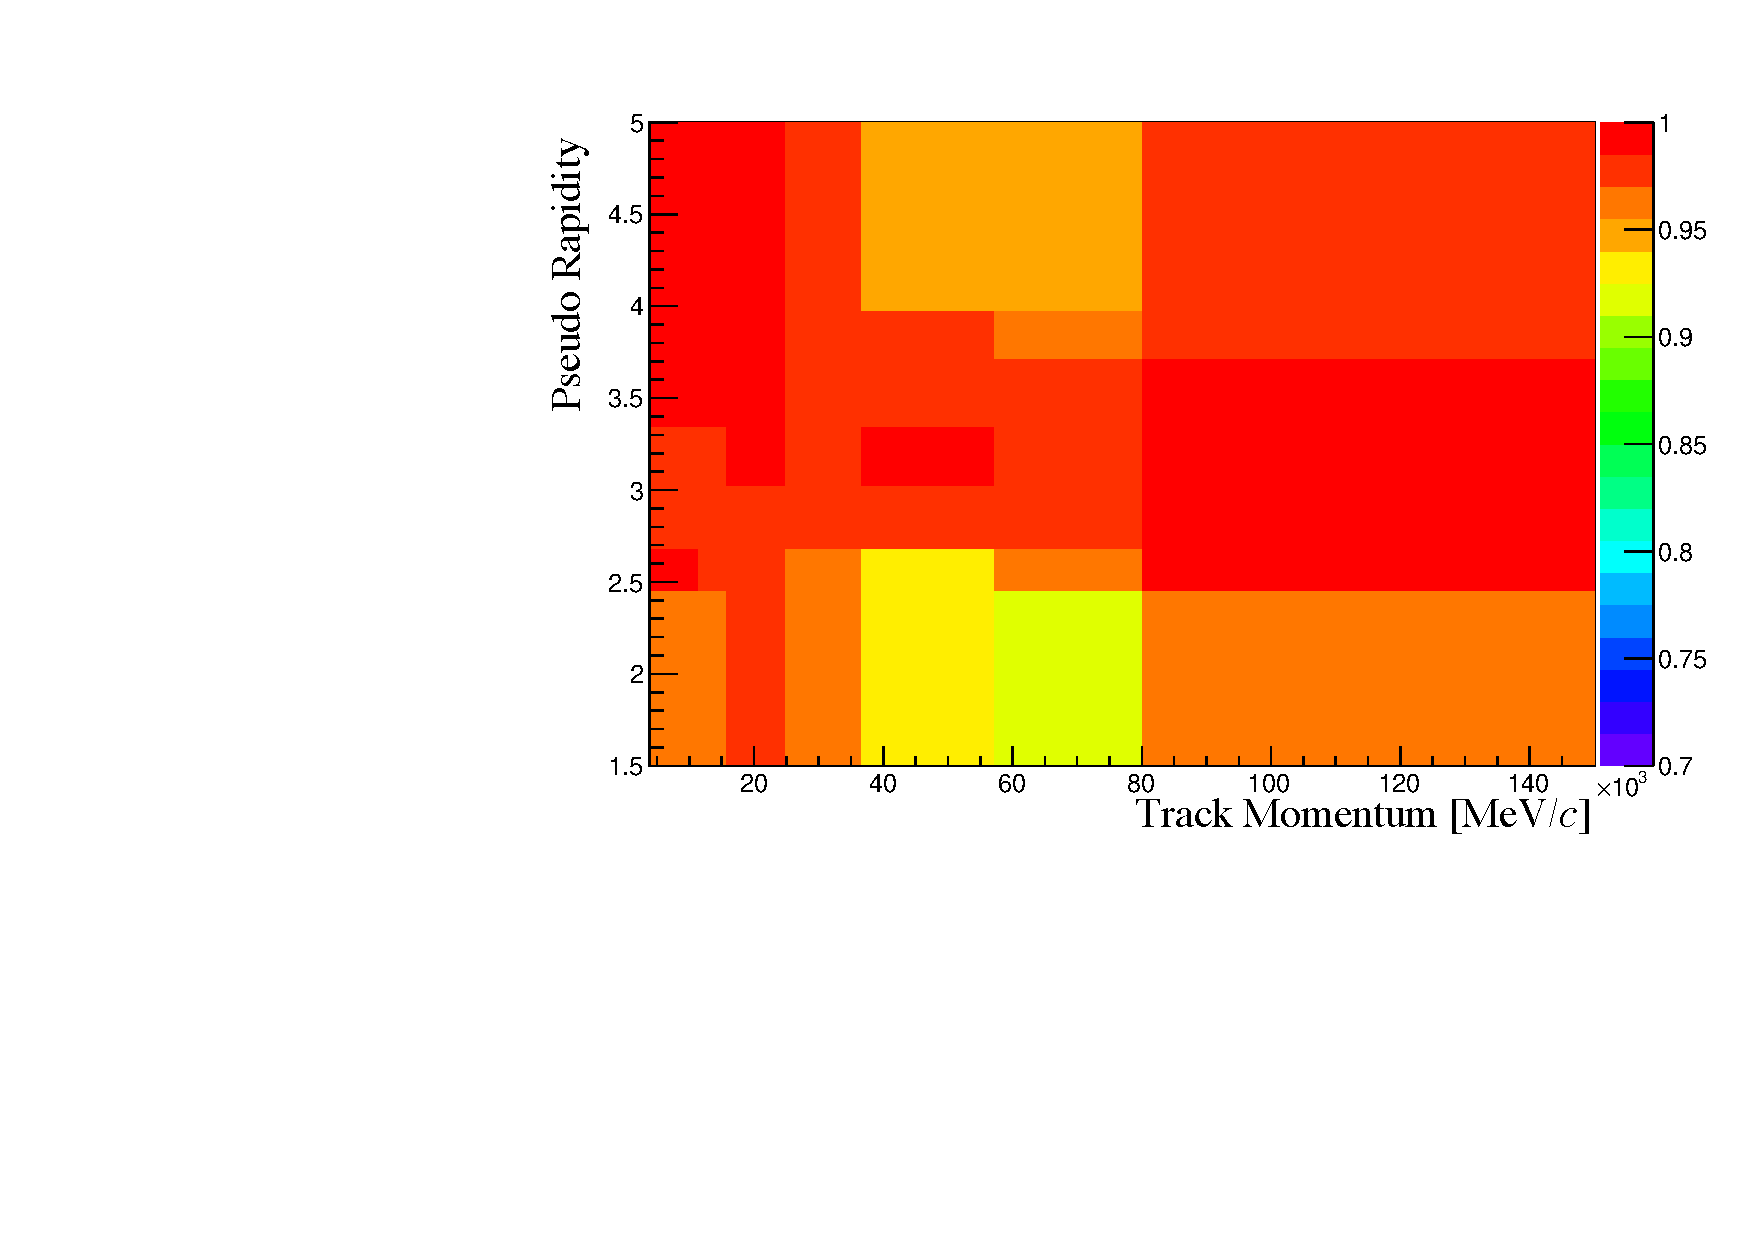
\includegraphics[width=0.49\textwidth]{RKst/figs/pid_Pi.pdf}
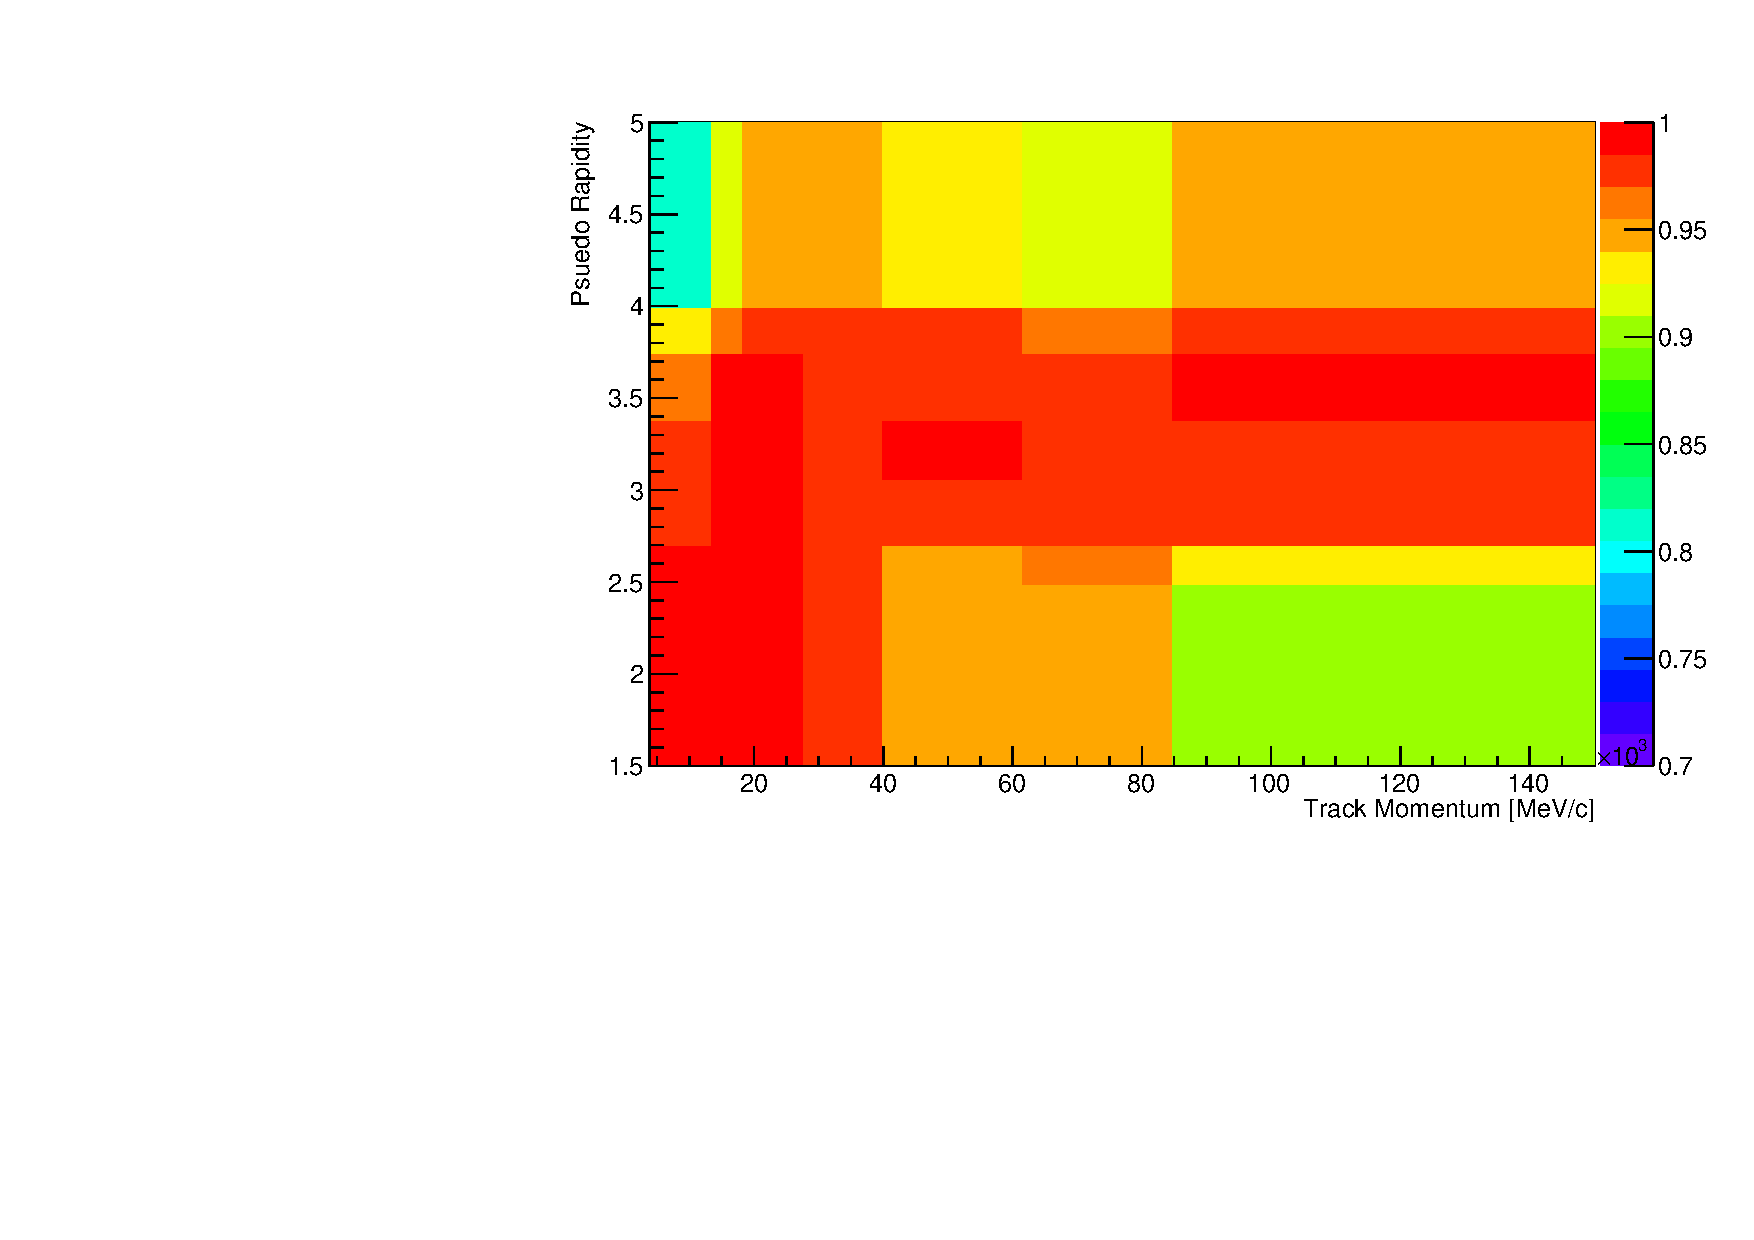
\includegraphics[width=0.49\textwidth]{RKst/figs/pid_K.pdf}
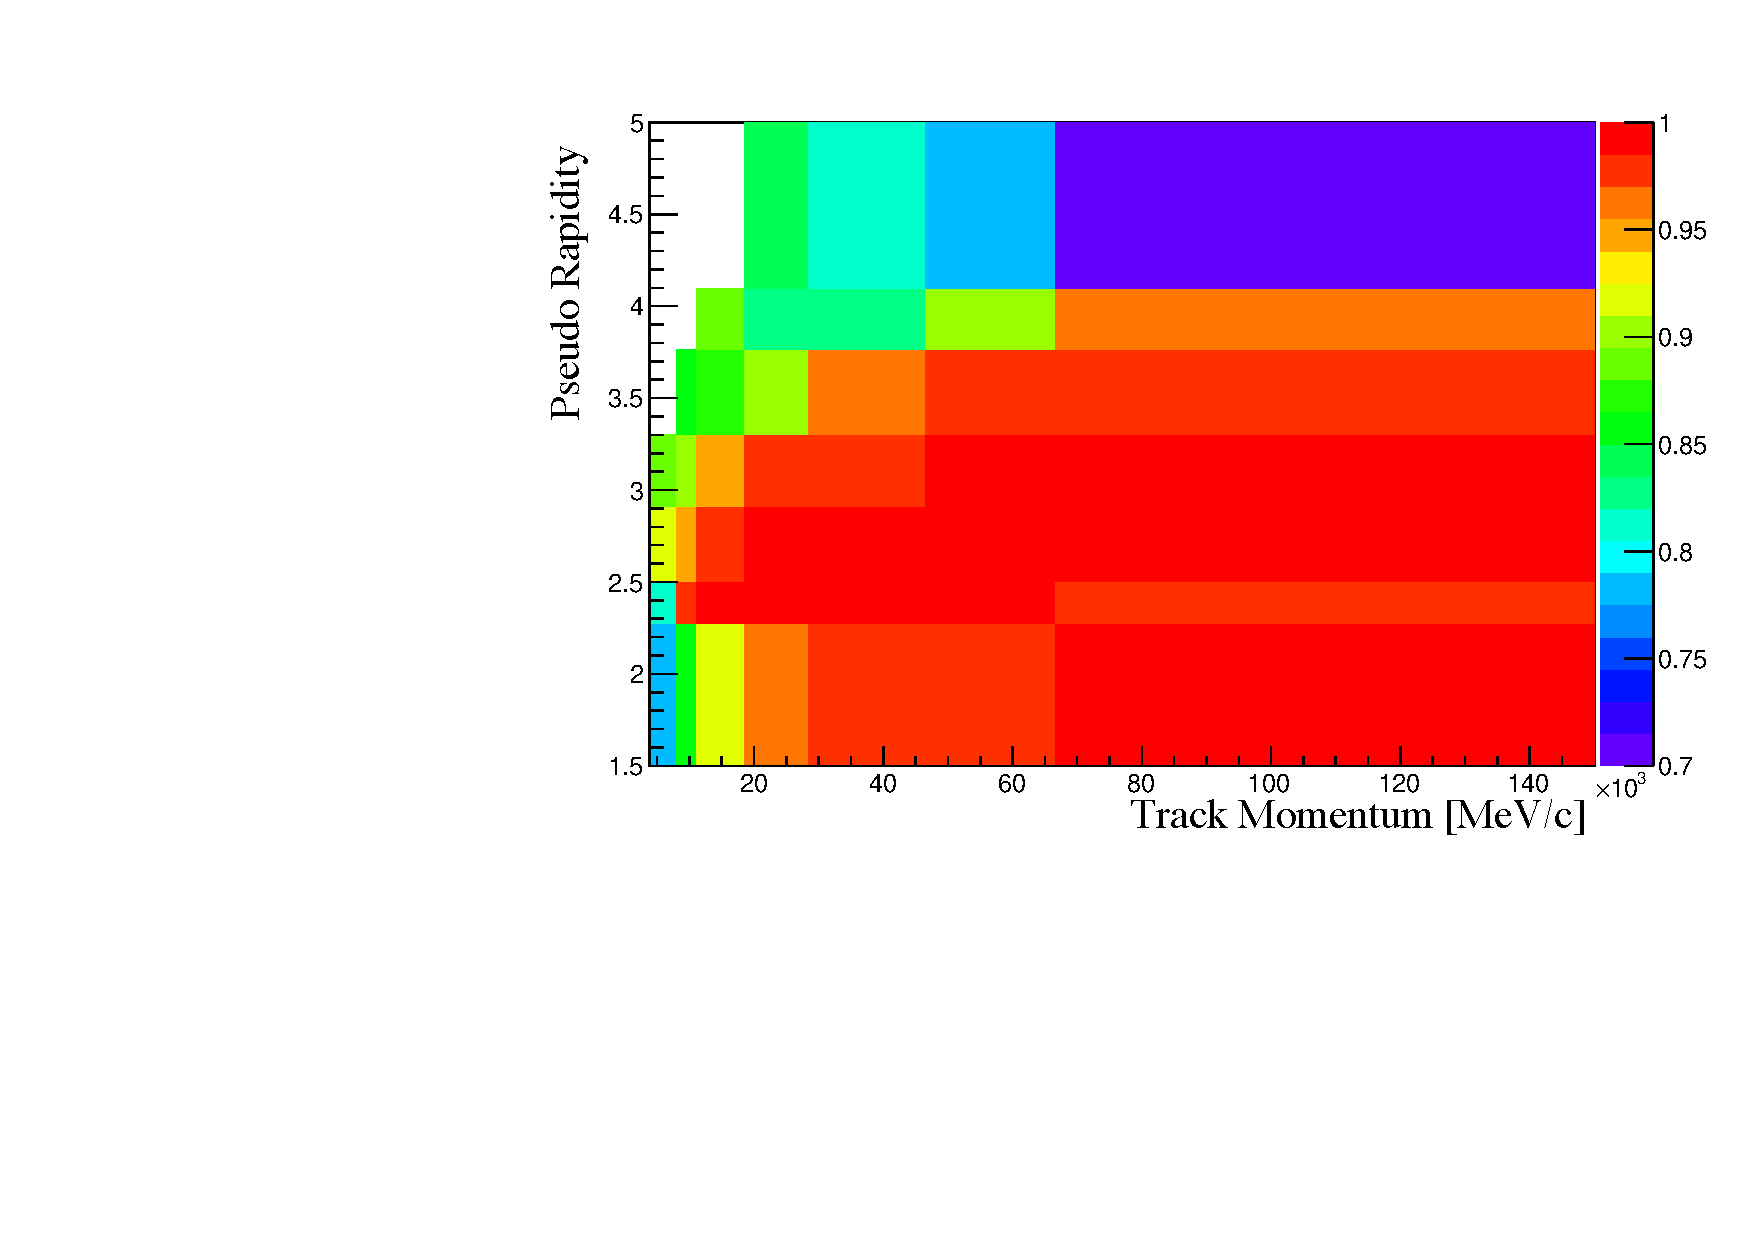
\includegraphics[width=0.49\textwidth]{RKst/figs/pid_Mu.pdf}
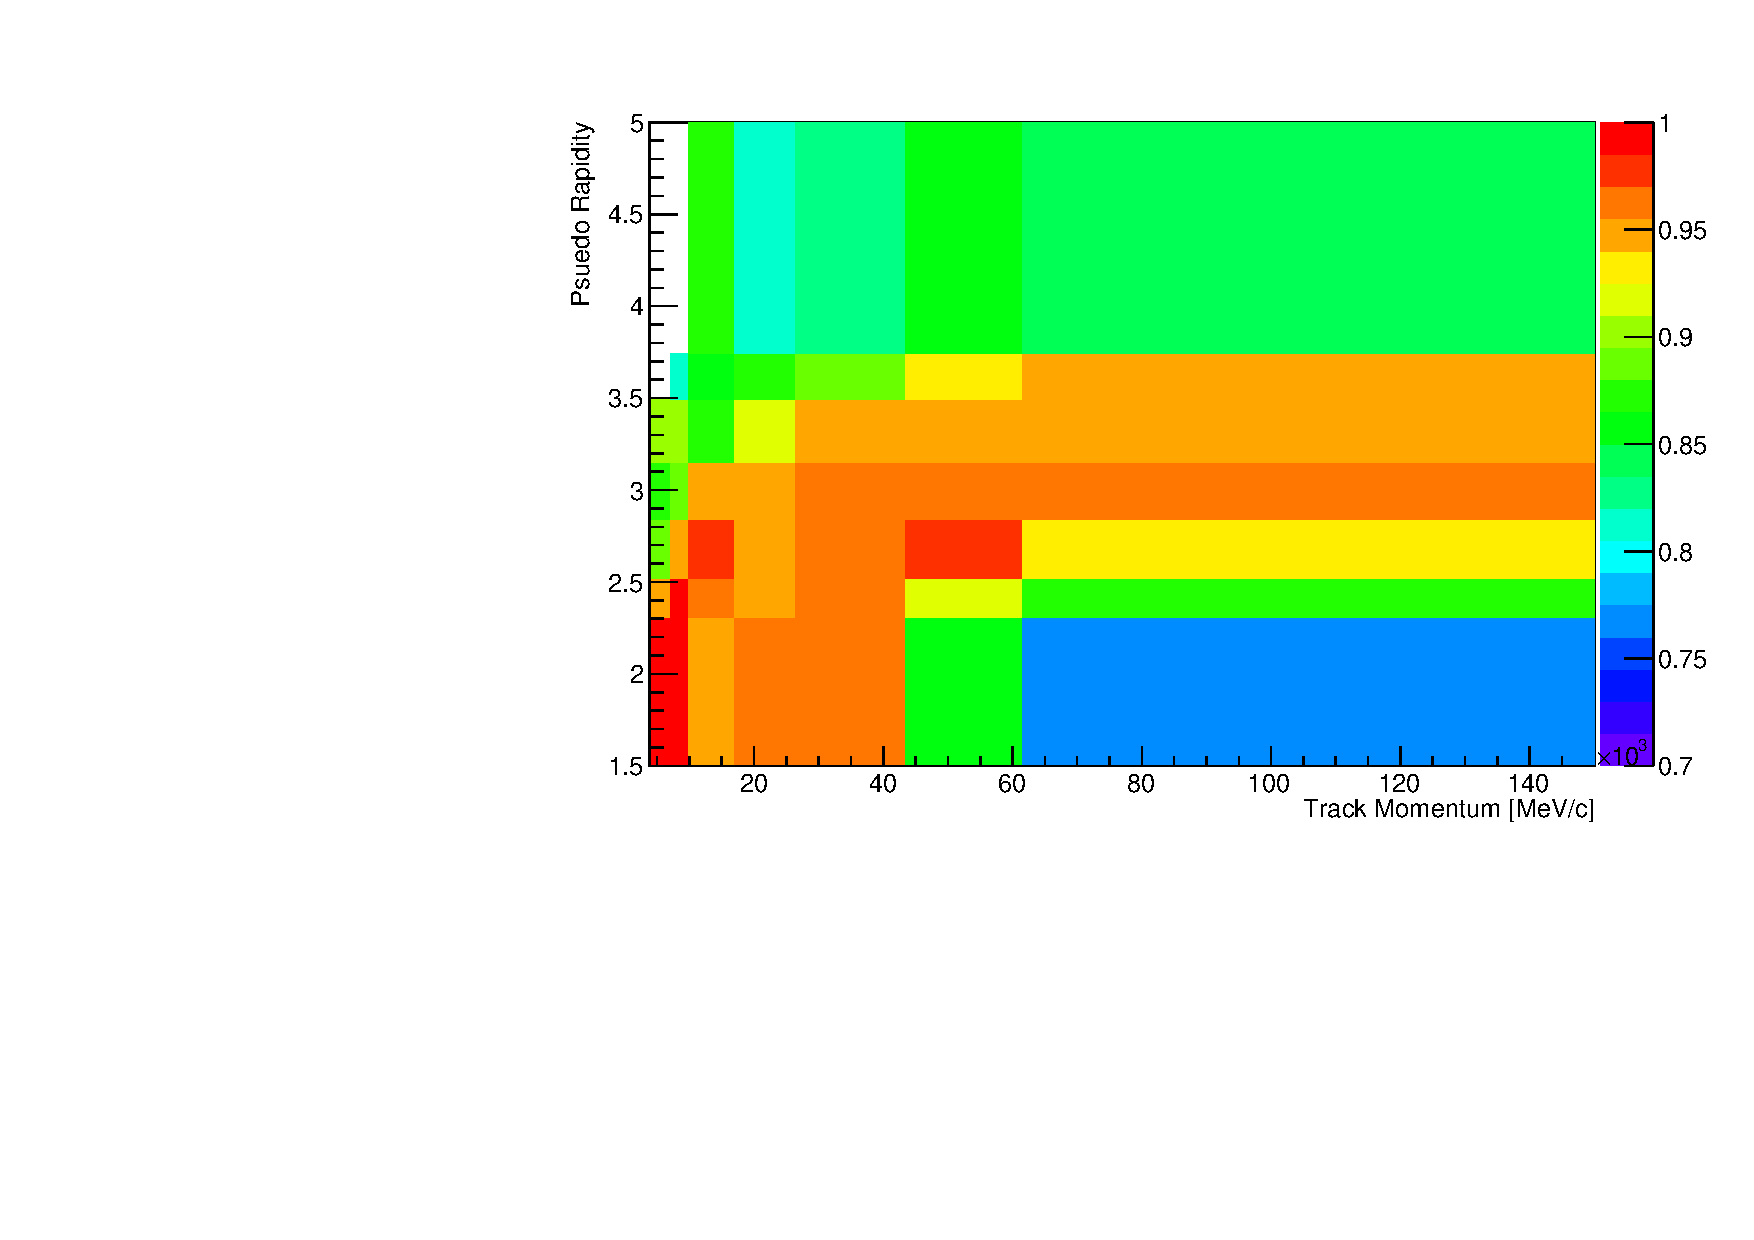
\includegraphics[width=0.49\textwidth]{RKst/figs/pid_e.pdf}
\caption{PID efficiency performance tables in regions of $\eta$~and $p$ of the particle under study, 
obtained with a data-driven method: for pions (top left), kaons (top right), muons (bottom left) 
and electrons (bottom right).}
\label{fig:pid_perf_hist}
\end{figure}


\subsection{Trigger efficiency}
\label{sec:RKst_trigger_eff}

While the trigger efficiency for the muon channels is calculated using simulated events,
for the electron channels a combination of simulation and data-driven methods is used.
The efficiency of the software stage, HLT, is always obtained from simulation,
while the efficiency of the hardware stage, L0, is obtained using a data-driven method
as described in the next subsection.
For both muon and electron channels it is possible to use the resonant sample to cross-check
the efficiency obtained using the simulation, as explained in Sec.~\ref{sec:tistos}.

\subsubsection{Electron triggers}
\label{sec:RKst_trigee}

For the electron channels data is fitted separately in three trigger categories: L0E, L0H and L0I
and therefore the efficiency is calculated separately for each category.
While the HLT1 and HLT2 efficiencies are derived using simulated events,
the efficiency for the L0Electron and L0Hadron triggers, based on calorimeter information,
 cannot be obtained from the simulation because the ageing of the calorimeters, which 
 modifies their response with time, is not simulated.
Therefore, in these cases the L0 trigger efficiency must be calibrated using data driven-methods.

Tables of efficiencies as a function of the \pt of the relevant particle for each trigger 
are obtained by applying the TISTOS method to a calibration sample.
%For each trigger category these tables contain the efficiency as a function of
%the \pt of the considered particle and are given for different calorimeter regions
These are given separately for calorimeter regions with different properties \emph{e.g.} the cell size.
%due to the different position with respect to the beam line. 
The considered regions are the inner and outer HCAL, 
and the inner, middle and outer ECAL. Figure~\ref{sec:L0eff_tables} shows data-driven 
efficiencies for the L0Electron trigger in the three ECAL regions as a function of the \pt of the electron.
%
\begin{figure}[h!]
\centering
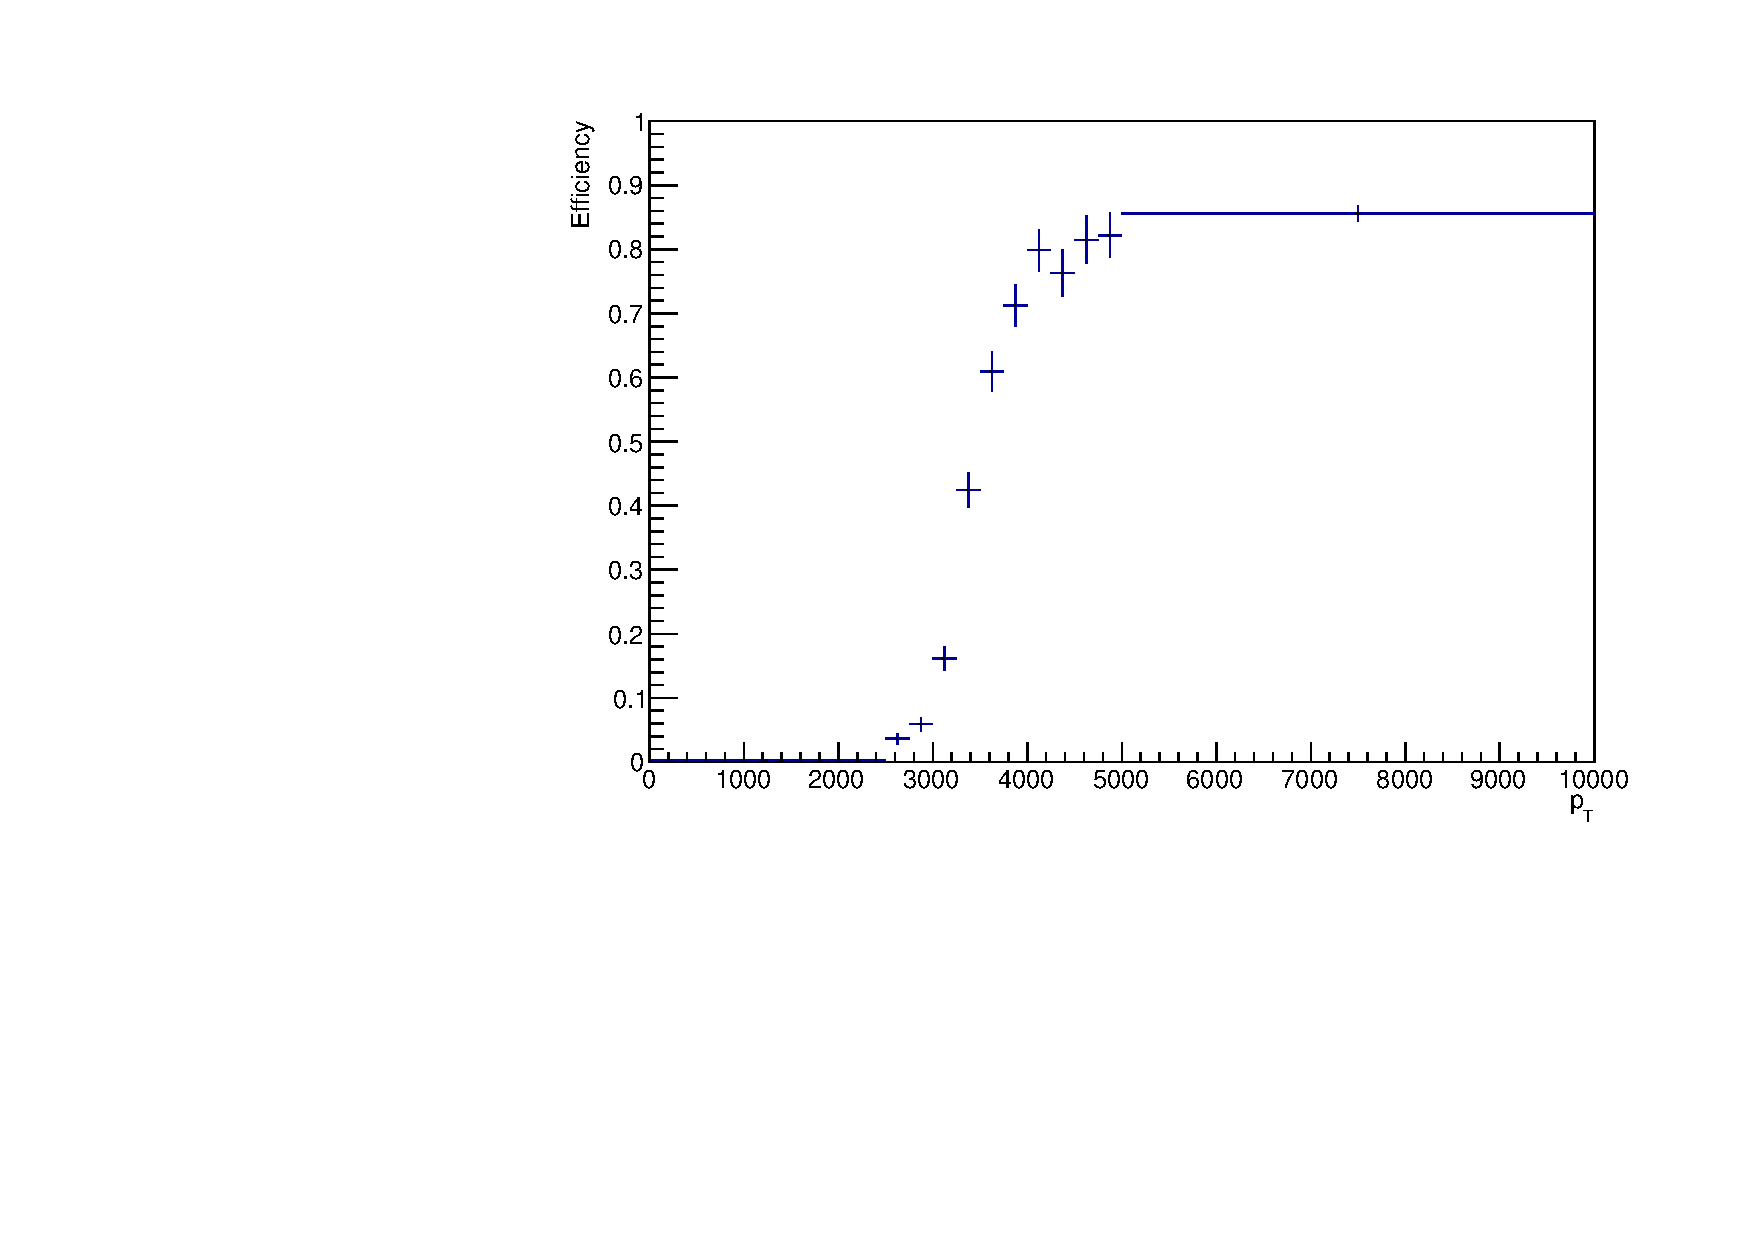
\includegraphics[width=0.49\textwidth]{RKst/figs/l0plots/l0E_Inner.pdf}
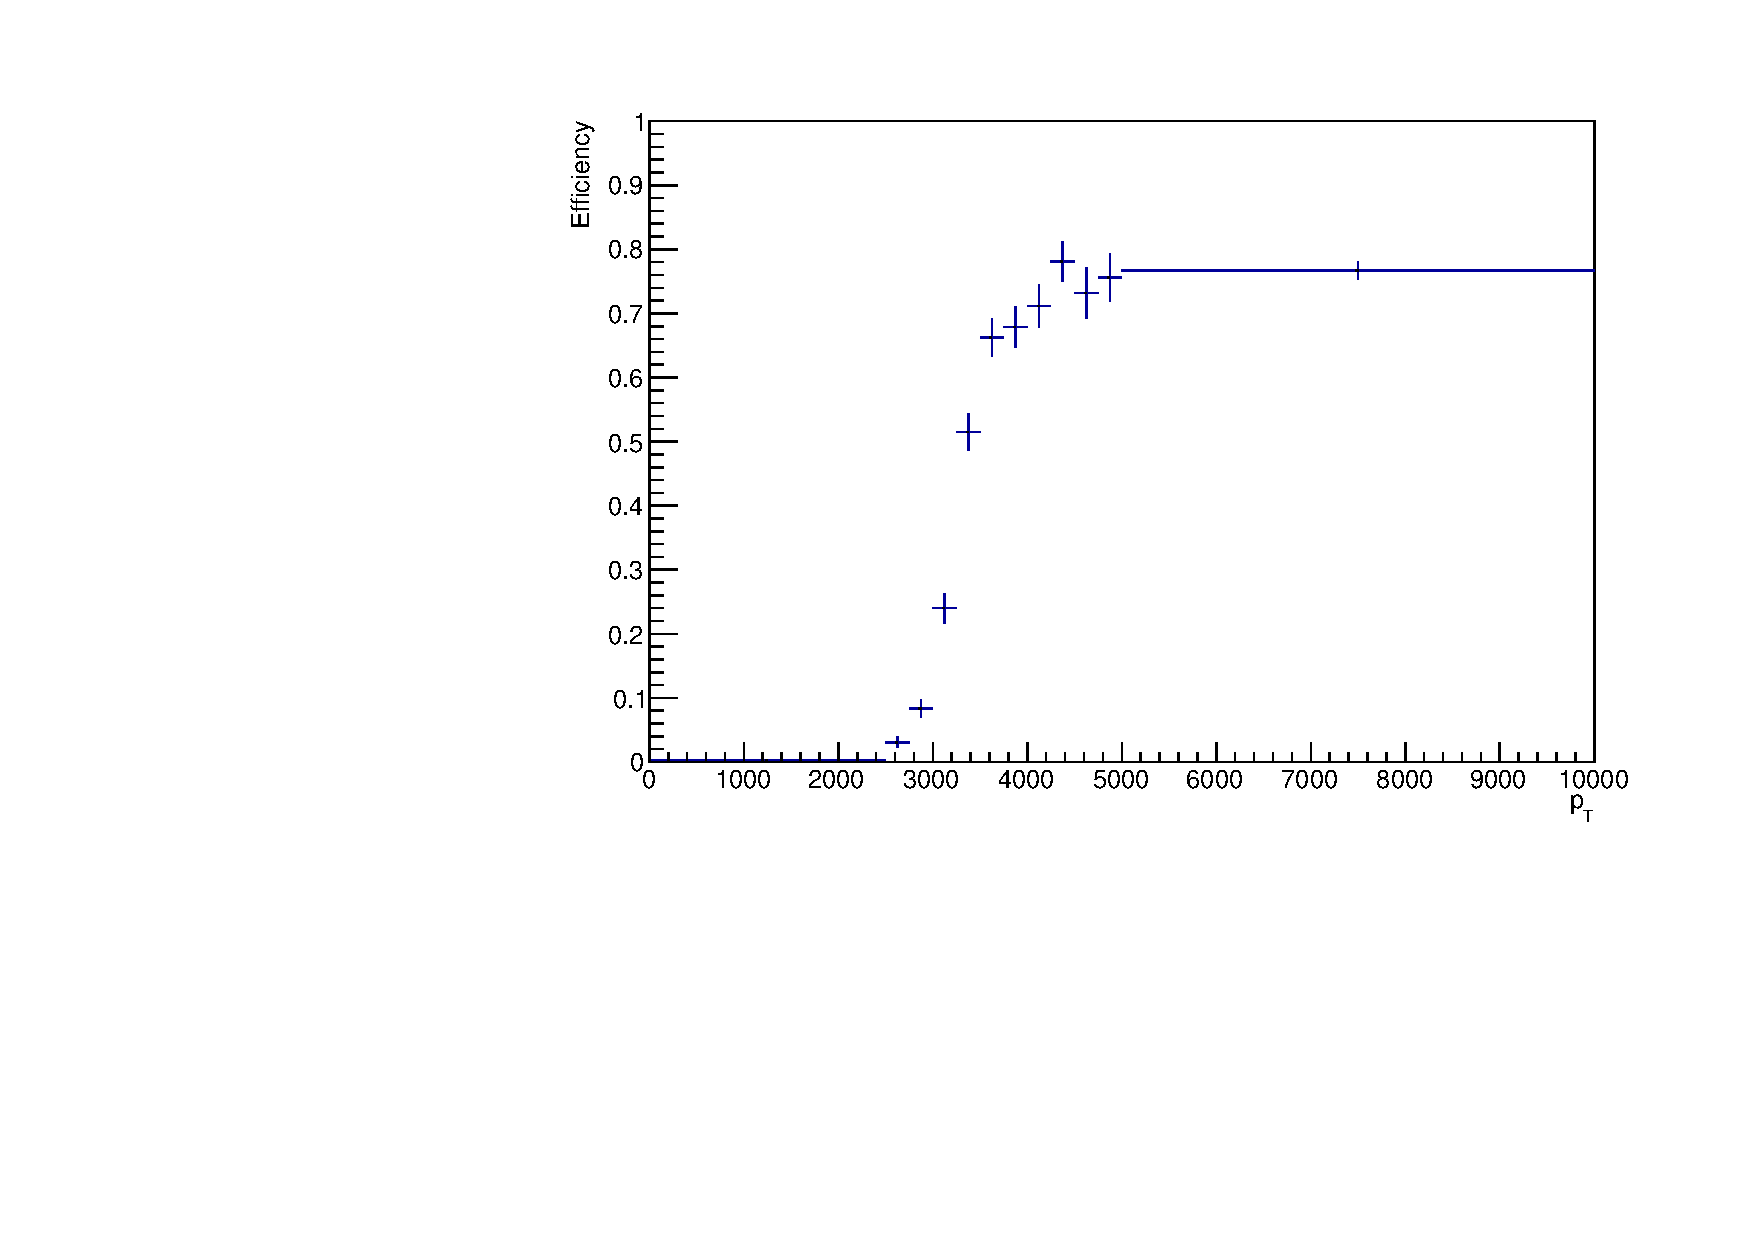
\includegraphics[width=0.49\textwidth]{RKst/figs/l0plots/l0E_Middle.pdf}
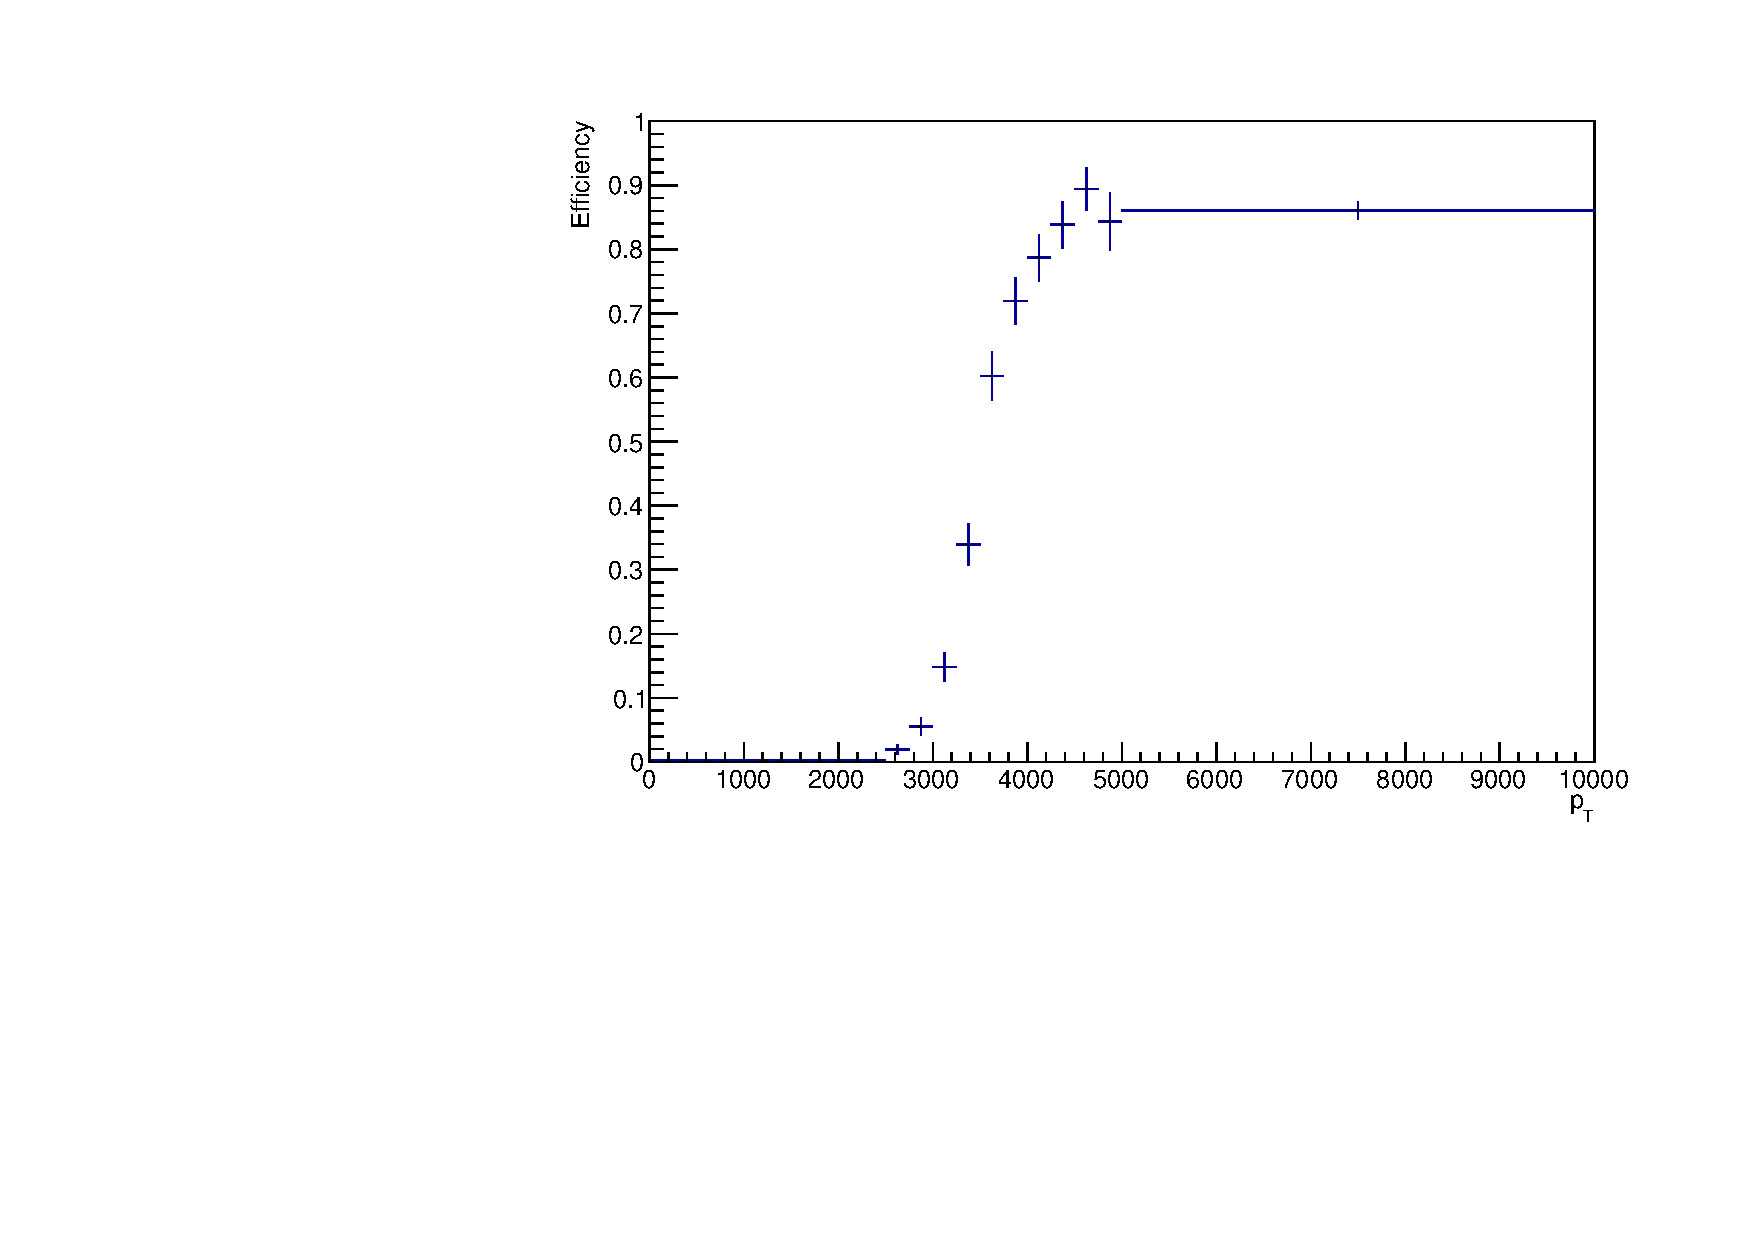
\includegraphics[width=0.49\textwidth]{RKst/figs/l0plots/l0E_Outer.pdf}
\caption{Data-driven L0Electron trigger efficiencies as a function of the transverse momentum
of the electrons for the three ECAL regions: inner (top left), middle (top right) and outer (bottom).}
\label{sec:L0eff_tables}
\end{figure}

The probabilities of an event being triggered by L0Electron or L0Hadron are calculated for each candidate as:
%
$$P_{L0E} = \varepsilon(e^+) + \varepsilon(e^-) - \varepsilon(e^+)\varepsilon(e^-) \text{ and }  
 P_{L0H} = \varepsilon(\pi) + \varepsilon(K) - \varepsilon(\pi)\varepsilon(K).$$
%
The probability of a TIS trigger is independent of the signal by definition and therefore 
must be the same in the rare and resonant channels and hence cancel in their ratio.

Event by event efficiencies for the three trigger categories are then defined to be exclusive in the following way:
%
\begin{itemize}
\item L0E: $\varepsilon^{L0E} = P_{L0E}$, namely the probability that the trigger decision is due to at least one of the electrons of a decay candidate;
\item L0H: $\varepsilon^{L0H} = P_{L0H}\cdot(1 - P_{L0E})$, namely the probability that the trigger decision is due to at least one of the hadrons of a decay candidate but none of the electrons;
\item L0I: $\varepsilon^{L0I} = (1-P_{L0H})\cdot(1 - P_{L0E})$, namely the probability that neither the hadrons or the electrons in decays 
candidates are responsible for the trigger decision. Note that in this case $\varepsilon^{L0I} $ does not correspond to the efficiency of 
TIS trigger but to the probability that the event does not fall into the L0E or L0H categories.
\end{itemize}
%
%The total efficiency for each category is then found by using the kinematic distribution from MC events,
%weighted for PID efficiencies, SPD and \Bz $p_T$ as described in \ref{sec:MCweighting}.
Finally, as in the PID case, the total efficiency is found by averaging over all events of a simulated sample:
%
\begin{equation}
\varepsilon^{\rm L0} = \frac{1}{N} \sum_i^N \varepsilon^{\rm L0}(\pt^i),
\end{equation}
\noindent
where ``L0" is a label indicating the trigger category under consideration.

\subsubsection{TISTOS cross-check}
\label{sec:tistos}

The efficiency obtained using the simulation is cross-checked by applying the \mbox{TISTOS}
 method, already described in Sec.~\ref{sec:Lb_trigger_eff}, to resonant data.
%
%In LHCb triggered events can fall in two categories: events triggered by a track which is part
%of the candidate decay of interest, Trigger On Signal (TOS), or by other tracks in the event,
%Trigger Independent of Signal (TIS). All trigger lines used for this analysis are required to be TOS.
%The TIS and TOS samples are not exclusive but independent. Therefore the efficiency for TOS
%trigger can be obtained by data by the following formula:
%\begin{equation}
%\varepsilon_{TOS} = \frac{TOS \mbox{ and } TIS}{TIS}
%\end{equation}
%
For this purpose a sample of \BdToKstJPsll candidates triggered independent-of-signal is used
as the control sample. As data also contains non-negligible amounts of background, 
%the \verb!DecayTreeFitter! tool is used to constrain the \jpsi mass to its known value and 
a narrow interval around the peak, dominated by the signal, is selected and the $_{s}\mathcal{P}lot$ method
is used to remove residual background in the data sample. 
Results are shown in Tab.~\ref{tab:tistos}, where the
efficiency obtained using the TISTOS method is compared between data and simulation.
These are found to be in agreement for the muon channel,
while they show deviations in the electron channels. In particular a significant discrepancy is found,
for the L0I category, for which the procedure explained in Sec.~\ref{sec:RKst_trigee} does not ensure
a correct calibration. The table also reports a correction factor
obtained according to the formula
\begin{equation}
f = 1 + \frac{\varepsilon_{data}^{\rm TISTOS} - \varepsilon_{MC}^{\rm  TISTOS}}{\varepsilon_{MC}^{\rm  TISTOS}},
\end{equation}
which can be used to correct the absolute resonant yields.
%
Although discrepancies are present, they are expected to cancel in the ratio between the rare and \jpsi channels;
only the residual discrepancy on this ratio, due to the different \qsq, is relevant for the measurement of \RKst.
In order to check if discrepancies do indeed cancel, a data-driven efficiency is
also required for the rare channels. To do this, the TISTOS efficiency obtained using \BdToKstJPsll candidates 
must be re-weighted to account for the different kinematics of the rare and resonant channels. This is done by determining
the TISTOS efficiency as function of the maximum \pt of the particles responsible for the L0 trigger decision, \emph{i.e.} 
the leptons for \verb!L0Electron! and \verb!L0Muon!, the kaon and the pion for \verb!L0Hadron!, and all final state 
particles for \verb!L0Global!. These efficiencies, shown in Fig.~\ref{fig:tistos_vs_pt}, are used to re-weight the 
distribution of simulated rare candidates.
%
%To check the effect of this correction on the ratios between rare and resonant channels,
%the efficiency obtained using the TISTOS method is plot as a function of the kinematic
%quantity relevant for each trigger category:
%the maximum \pt of the electrons for L0E, the maximum \pt of $K$ and $\pi$ for L0H,
%and the maximum \pt of all the final particles for L0I; results are shown in Fig.~\ref{fig:tistos_vs_pt}.
%The \pt distributions of the rare and resonant simulated samples are then used to find
%the average efficiency in the two cases. This corresponds to making an average of the efficiency
%weighted by the kinematical distributions in the two samples. 
%
The ratios $\varepsilon^{\rm TISTOS}_{\ell\ell} / \varepsilon^{\rm TISTOS}_{\jpsi}$ obtained using the data-driven method
and simulation are compared and found to be fully compatible. This means that, even though
the TISTOS correction has an effect on the absolute efficiency of each channel, this is negligible on their ratio 
as originally anticipated. Therefore, no correction due to this effect is applied for the calculation of the \RKst ratio.
%
\begin{table}[t]
\begin{center}
 \caption{Trigger efficiencies obtained using the TISTOS method on
 simulated and real $\decay{\Bz}{\Kstarz\jpsi(\to\ell^+\ell^-)}$ decays.}
\begin{tabular}{$c|^c^c^c}
\rowstyle{\bfseries}
 Sample 					&  MC  			     & Data 			   & Correction factor		\\ \hline
$ J/\psi \rightarrow \mu\mu$      & $ 0.797  \pm  0.002 $ & $ 0.803  \pm  0.004 $   &  1.0073  \\
$J/\psi \rightarrow ee$ L0E     	& $ 0.268  \pm  0.002 $ & $ 0.255  \pm  0.004 $   &  0.9536   \\
$J/\psi \rightarrow ee$ L0H     	& $ 0.028  \pm  0.001 $ & $ 0.026  \pm  0.002 $   &  0.9269   \\
$J/\psi \rightarrow ee$ L0I     	& $ 0.017  \pm  0.001 $ & $ 0.011  \pm  0.001 $   &  0.6760   \\
  \end{tabular}
\label{tab:tistos}
\end{center}
\end{table}
%
\begin{figure}[h!]
\centering
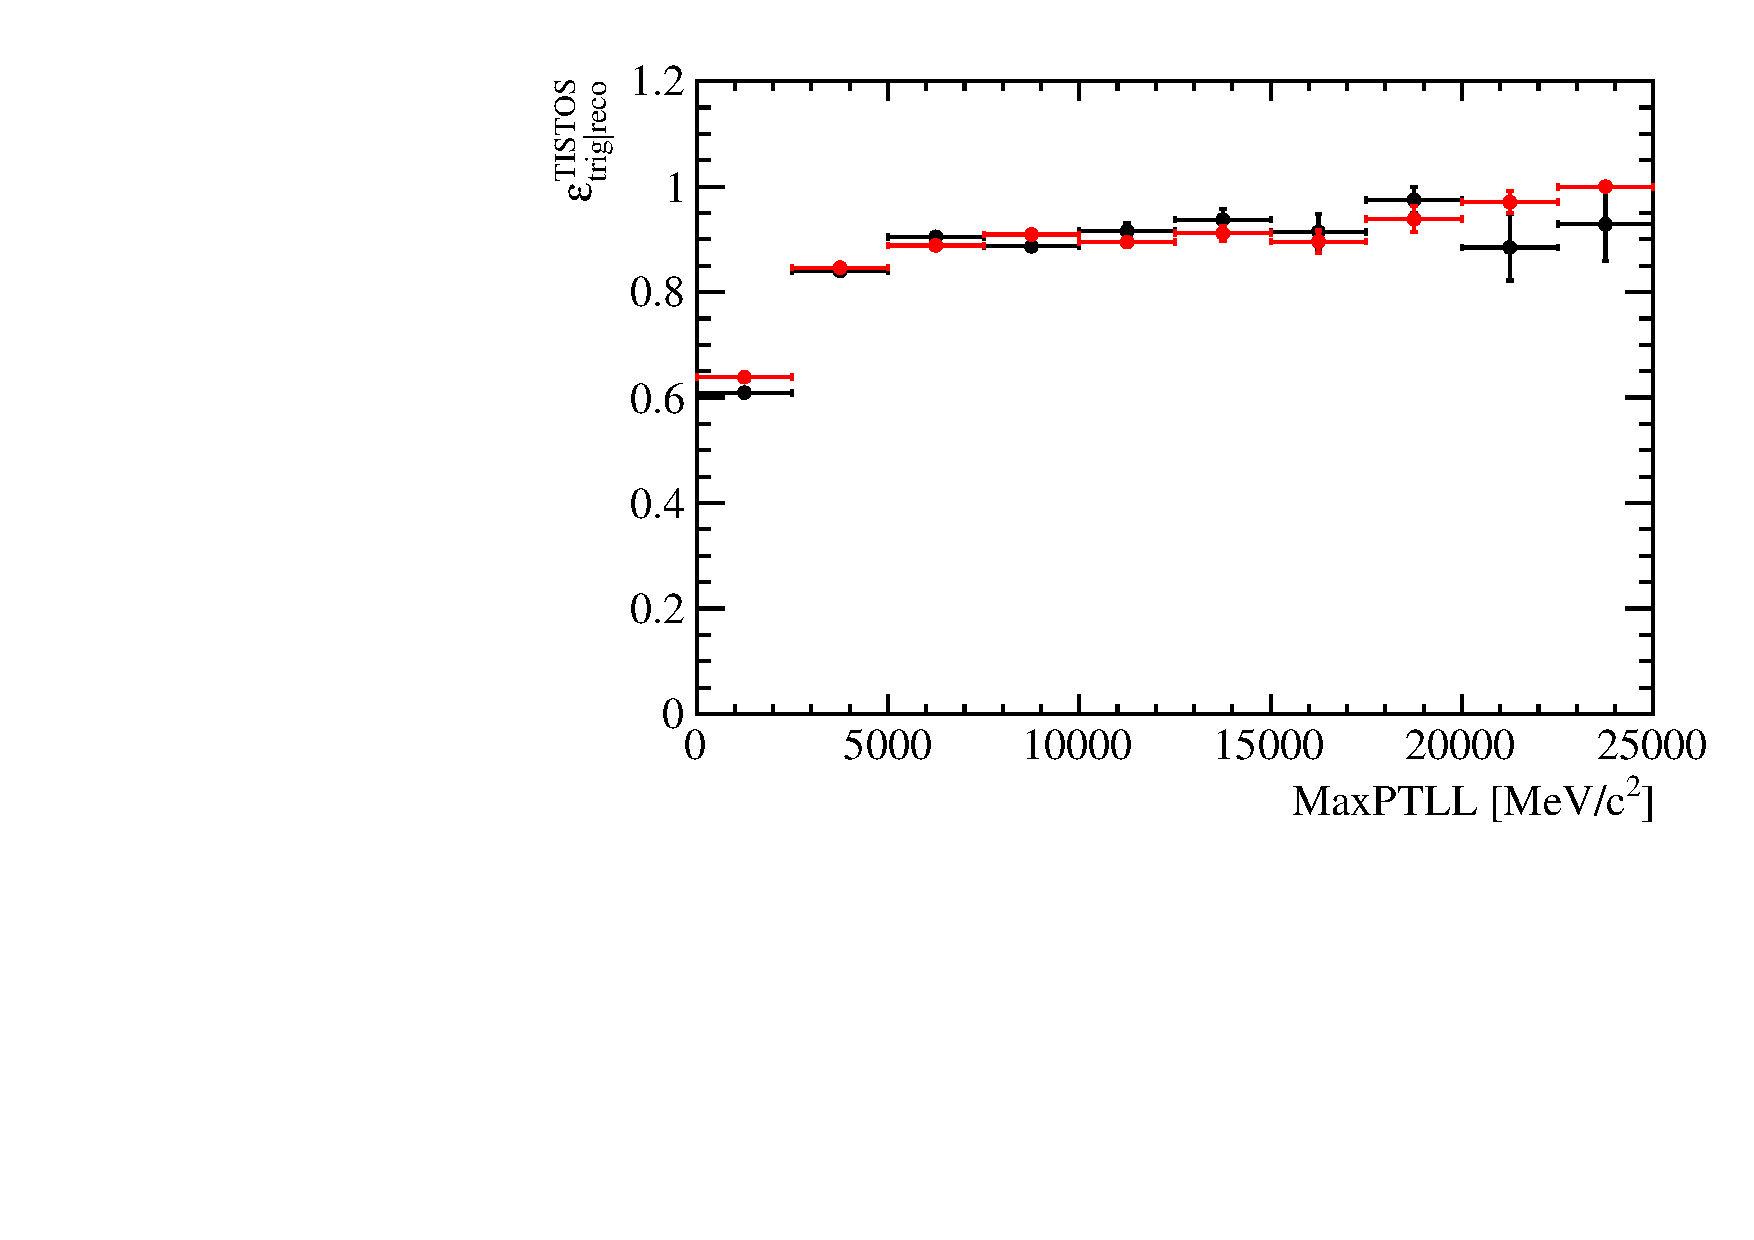
\includegraphics[width=0.49\textwidth]{RKst/figs/Efficiencies/efficiencyTisTos_MM.pdf}
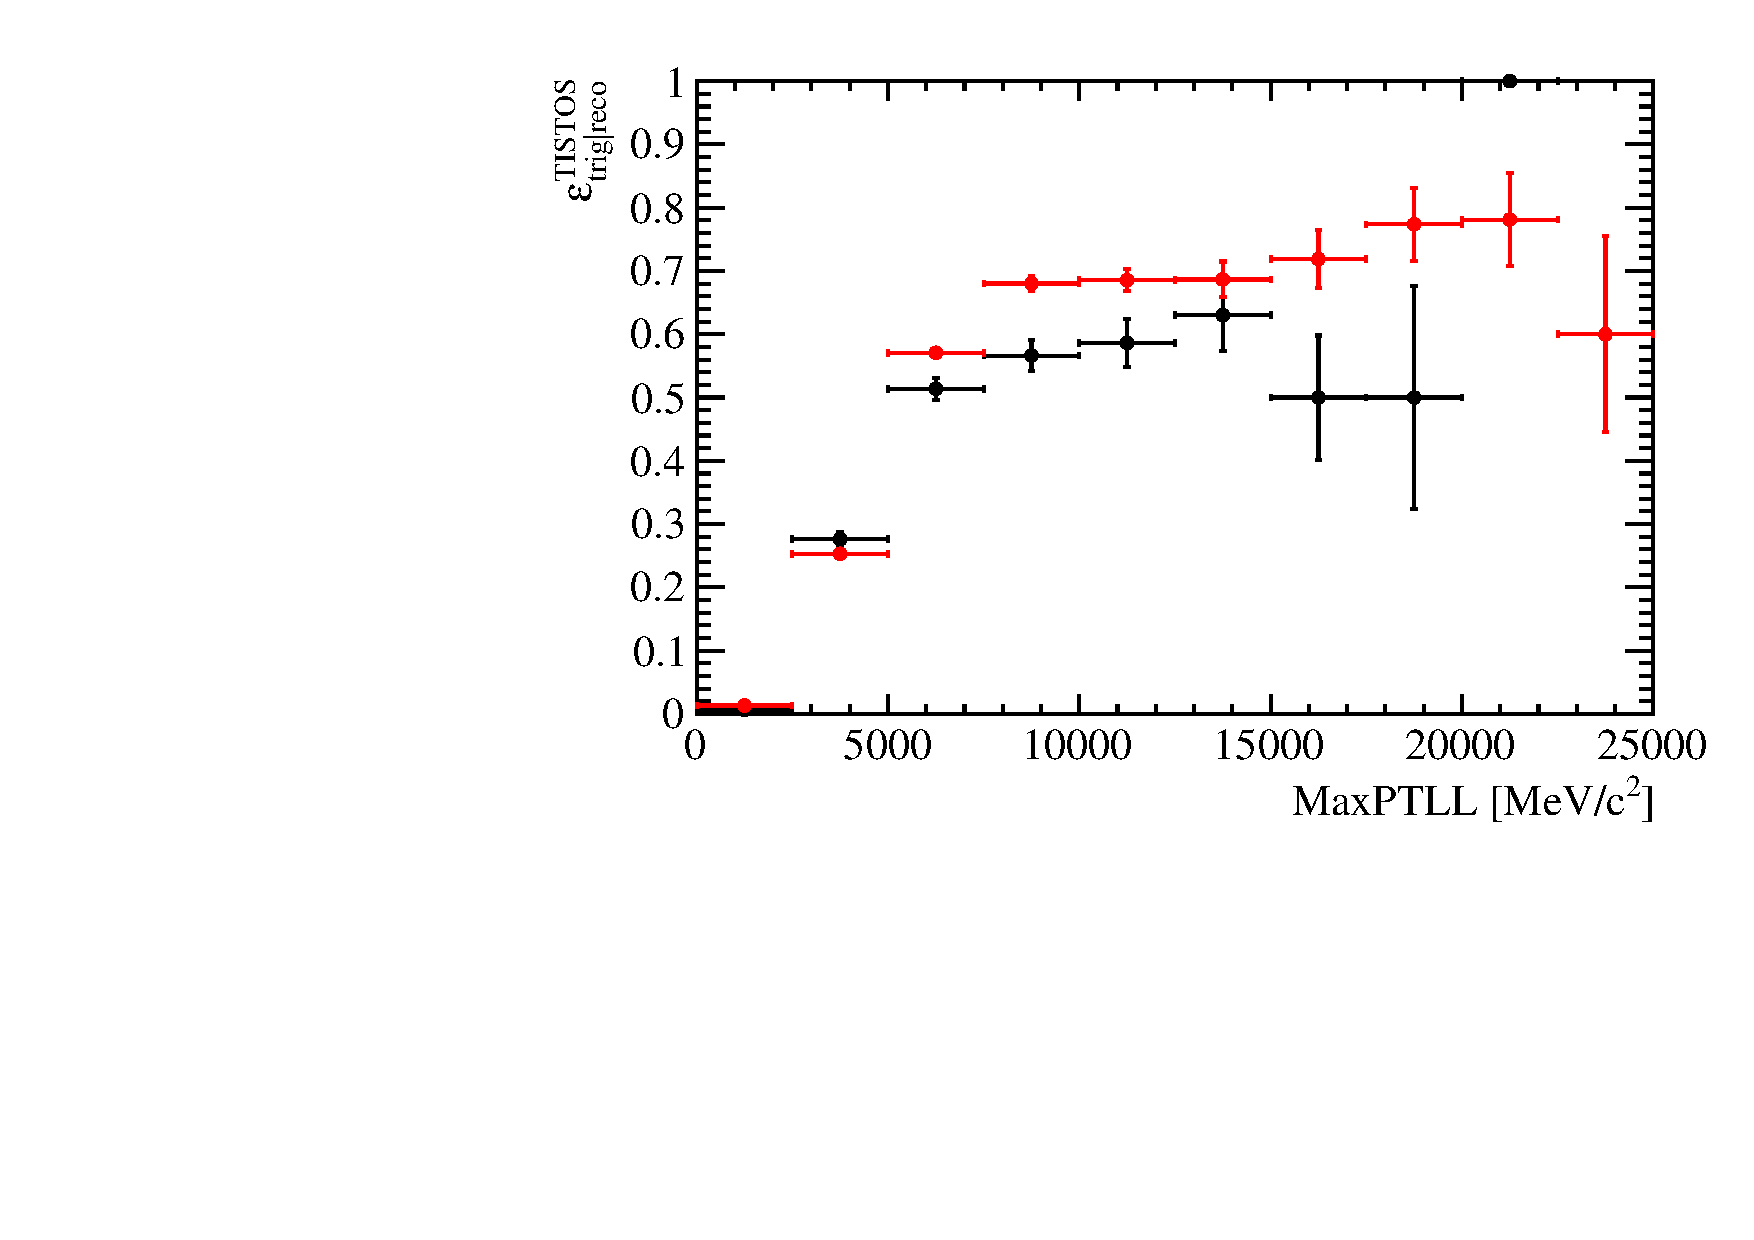
\includegraphics[width=0.49\textwidth]{RKst/figs/Efficiencies/efficiencyTisTos_EE_L0E.pdf}
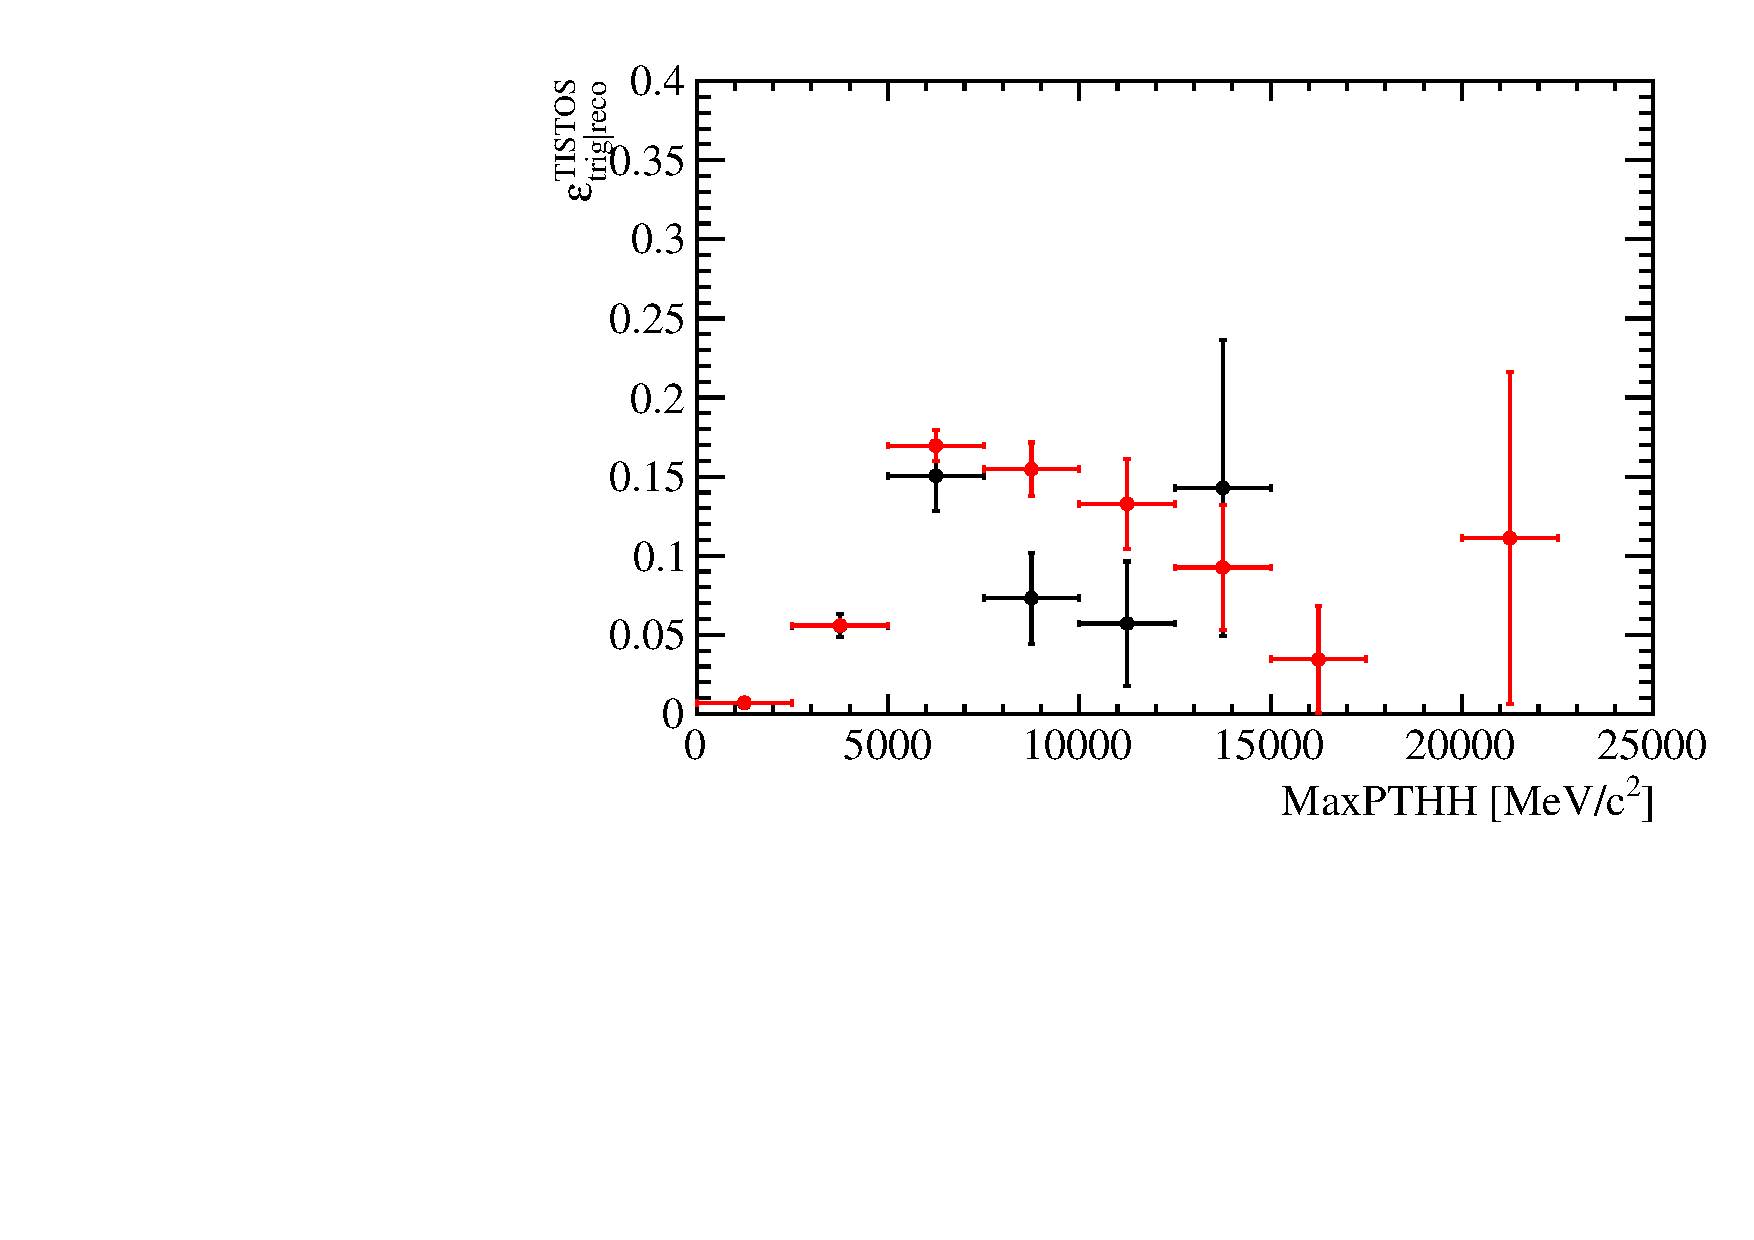
\includegraphics[width=0.49\textwidth]{RKst/figs/Efficiencies/efficiencyTisTos_EE_L0H.pdf}
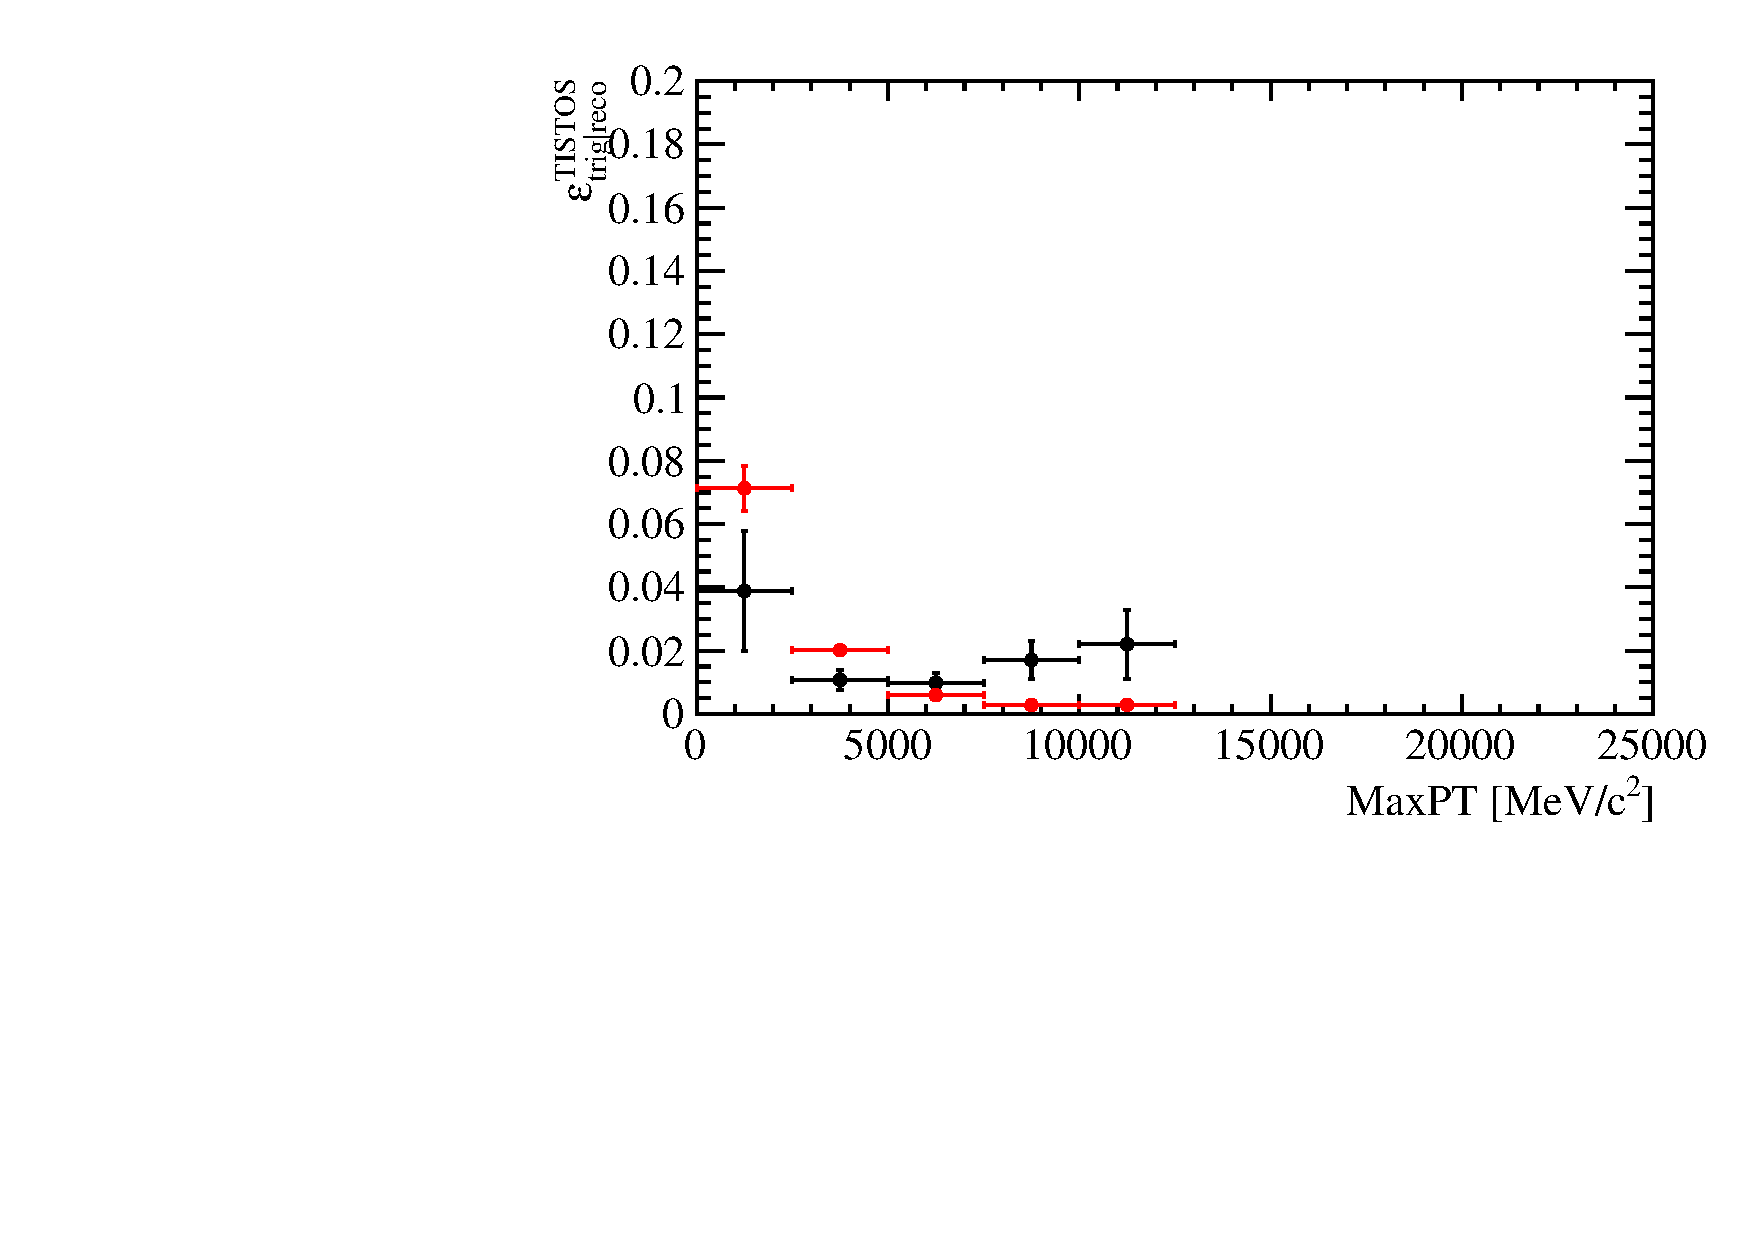
\includegraphics[width=0.49\textwidth]{RKst/figs/Efficiencies/efficiencyTisTos_EE_L0I.pdf}
\caption{Trigger efficiency obtained by applying the TISTOS method to \mbox{\BdToKstJPsll} candidates
as a function of the maximum \pt of the two muons (top left), the maximum \pt of the two electrons for the L0E category (top right), 
the maximum \pt of $K$ and $\pi$ for L0H (bottom left) and the maximum \pt of all the final particles for L0I (bottom right).}
\label{fig:tistos_vs_pt}
\end{figure}


\subsection{Neural networks and BCM efficiencies}
\label{sec:Rkst_mva_eff}

The neural network and BCM efficiencies are evaluated from fully weighted simulated samples,
and separately for each trigger category for the electron channels.
%, because the yield is extracted independently for each of the three trigger categories
%and therefore these have to be independently corrected.
%
To check for biases the efficiency obtained for \mbox{$\decay{\Bz}{\Kstarz(\jpsi\to\ll)}$} decays can 
be compared with that obtained for rare $\decay{\Bz}{\Kstarz \ll}$ decays
selected in the same \qsq region used for the resonant case. The ratio between the two should
be close to unity with small deviations due the fact that the \qsq interval has a finite width and the events
are distributed differently within the interval. This ratio is found to be $ 0.997  \pm  0.004 $ for the
$\mu\mu$ channels and $0.981  \pm  0.005$ for the $ee$ channels.
Values for the electron channels show a small deviation from unity due to the very large
\qsq interval used to select the resonant channel (6 -- 11~\gevgevcccc).

%\begin{table}[h!]
%\begin{tabular}{|c|c|c|c|c|}
%\hline Comp 			&  $\mu\mu$  				& \multicolumn {3}{c|}{$ee$}  \\ \hline
%				&   &  L0E 	& L0H 	& L0I \\ \hline
%rec  & $ 1.0104  \pm  0.0095 $ & \multicolumn{3}{c|}{$ 1.1040  \pm  0.0034 $} \\ 
%\hline
%trg  & $ 1.0113  \pm  0.0055 $ & $ 0.9752  \pm  0.0063 $ & $ 1.0078  \pm  0.0248 $ & $ 0.9766  \pm  0.0113 $ \\ 
%mva  & $ 0.9969  \pm  0.0039 $ & $ 0.9771  \pm  0.0023 $ & $ 0.9794  \pm  0.0019 $ & $ 0.9856  \pm  0.0057 $ \\ 
%\hline
%\end{tabular}
%\caption{Ratio $\varepsilon^{\ell\ell} / \varepsilon^{\jpsi}$ where the efficiency for the
%rare channel is calculated in the same \qsq range used to select the resonant channel.}
%\label{tab:mva_in_jpsibin}
%\end{table}


%\clearpage








